\documentclass[10pt,twocolumn]{article}

\usepackage[T1]{fontenc}
\usepackage{lmodern}
\usepackage[margin=0.75in]{geometry}
\usepackage{amsmath,amssymb}
\usepackage{booktabs}
\usepackage{graphicx}
\usepackage{tikz}
\usepackage{pgfplots}
\pgfplotsset{compat=1.18}
\usetikzlibrary{arrows.meta,positioning,fit,backgrounds}
\usepackage[colorlinks=true,allcolors=blue]{hyperref}
\usepackage{microtype}
\usepackage{xcolor}

% One palette for every figure, so the paper reads as a single system. The three
% categorical hues clear a colourblind-separation check on all pairs (worst
% protan/deutan/tritan dE 8.1 in OKLab x100) and all three exceed 3:1 contrast
% against the page. Marker shape is varied alongside hue so identity never rests
% on colour alone.
\definecolor{gwelblue}{HTML}{1F3BE0}
\definecolor{gwelorange}{HTML}{C2570A}
\definecolor{gwelteal}{HTML}{00806A}
\definecolor{gwelgrid}{HTML}{D8D8D6}

\title{\vspace{-2em}\textbf{A Better Signal Is Not a Better Router:\\
Pre-Generation Escalation Decisions in Sub-Billion VLMs}\vspace{-0.5em}}
\author{Theophile Avenel\\
\small\href{https://github.com/thekester/gwel}{github.com/thekester/gwel}}
\date{}

\newcommand{\answerlow}{\textsc{Answer-Low}}
\newcommand{\crop}{\textsc{Crop}}
\newcommand{\ocr}{\textsc{Ocr}}

\begin{document}
\maketitle

\begin{abstract}
Vision--language cascades answer from a downsampled image and escalate to full
resolution when the model appears uncertain. Every published escalation policy
learns this decision by reinforcement learning on 7B-class models, and reads it
from the model's output distribution after generation. We ask what a
500M-parameter model already knows, before it writes a token.

Output confidence answers the wrong question. It predicts whether the cheap pass
will be \emph{correct} (AUROC $0.758$) and barely predicts whether escalating
would \emph{recover} a failed query ($0.617$), which is the quantity that
actually spends budget. The distinction is invisible for text LLMs, where the
intervention is extended reasoning over an unchanged input, and material here,
where it adds information the model has not seen.

A linear probe on pre-generation activations reads that quantity better
($0.760$). \textbf{Then it fails an audit we ran on ourselves, and that failure
is the paper's main result.} Escalation value is dataset-determined, DocVQA
repairs $45\%$ of its queries and VQAv2 $5\%$, and image size tracks the same
split, so raw image size, a feature costing no forward pass, reaches $0.748$.
Trained and tested inside one dataset the probe reaches $0.572$ where output
entropy, fitted on nothing, reaches $0.663$; it improves with data and never
closes the gap, at any depth, with any of four probe families including
non-linear ones. \textbf{The probe is largely a domain detector}: where it and
entropy disagree, the disagreement predicts which dataset a query came from at
AUROC $0.738$. On a benchmark mixture it routes well; on the homogeneous
workload a deployment serves, the signal it beat is the better one.

The method survives the signal. Calibrating a score to the \emph{expected signed
gain} and thresholding at the break-even implied by measured latencies gives a
policy with no rate to tune, cost-optimal among policies that see only the score
(Proposition~1). Run on output entropy inside each domain, one unchanged
operator preference yields escalation rates from $1\%$ to $61\%$ that track what
escalation is worth there ($r = 0.974$), and dominates a fixed tuned rate.
Calibrating the weak pass's error probability instead, which is the standard
cascade recipe and coincides with ours exactly when escalation cannot hurt,
spends $59\%$ more compute for the same answers.

How far to escalate matters more than whether. On $1200$ document pages with
rungs chosen by measuring the model's patch-grid buckets, $93\%$ of what
escalation repairs is repaired below the top rung, and the top step gains
$-0.002\ [-0.026, +0.022]$ for $156$\,ms. That ceiling holds across an
$8.6\times$ parameter range and two distinct vision encoders, at the same pixel
resolution but different token counts, so it is a property of the pages rather
than of the model, and can be measured once per corpus.

The same signal does not say \emph{where} to look. A localizer pooling
visual-token states over candidate crops beats random cell choice at the finest
grid we test, at every depth, by $0.9$ accuracy points: $6\%$ of the gap a
perfect localizer would close. That gap is worth having, since at matched token
budget the best crop beats the dearest resolution setting at $2.5\times$ fewer
tokens.

Every comparison here is a cost comparison, so we measure the cost model rather
than assume it, and four standard proxies mispredict: the vision encoder is
$43\text{--}50\%$ of the visual cost, capping post-encoder pruning at half;
decode latency tracks depth rather than parameters; a flat per-configuration
price understates escalation by $16\%$; and on $56\%$ of the pilot the
``full-resolution'' configuration is not a distinct configuration at all. It was
that third correction, not a literature review, that exposed the domain
confound. Fifty-six claims, including the negative ones and the limits of the
positive ones, are re-derived from the data by a harness that fails loudly when
any stops holding, with paired comparisons corrected for family-wise error.
\end{abstract}

\section{Introduction}

A vision--language model asked ``what does the sign say?'' can answer from a
thumbnail or from the full-resolution image. The thumbnail costs a fraction as
much and is often sufficient. Deciding \emph{per query} which to use is the
premise of adaptive visual perception, and the premise is sound: on our pilot,
$34\%$ of queries are answered correctly at $384$\,px and would gain nothing
from more pixels, while $41\%$ fail at both resolutions and would gain nothing
either. Escalation changes the answer on $21\%$.

Published systems make this decision by learning it and by reading it after
generating: VisionThink~\cite{visionthink}, AdaptVision~\cite{adaptvision} and
AwaRes~\cite{awares} all train an escalation policy with reinforcement learning
on 7B-class models, supervised by judge models of their own.

Below one billion parameters none of that is available. Curating twenty
thousand samples and running GRPO is not an option for a model that exists
because it fits in a gigabyte of GPU memory~\cite{smolvlm}. Our question is
therefore narrow: \emph{what does a 500M VLM already know about its own need
for more pixels, and how cheaply can that be read?}

Fig.~
ef{fig:method} is where we end up: a single cheap pass, a score, and a
choice among resolution rungs priced by measured latency. The short answer
changed while we were writing it. On a benchmark mixture the
model appears to know more than its output reveals; on a single workload most of
that apparent knowledge turns out to be a recognition of which benchmark the
query came from. What survives is narrower and, we think, more useful: reading
the right quantity matters more than reading it well, deciding \emph{how far} to
escalate matters more than deciding \emph{whether}, and what the model knows is
whether to look again rather than where.

\begin{figure*}[t]
\centering
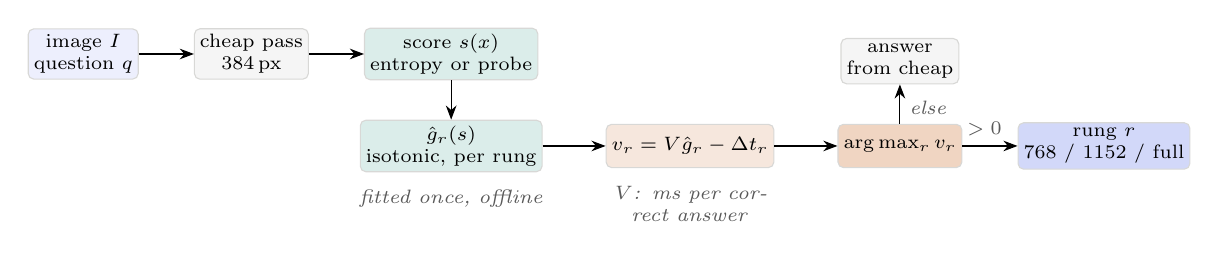
\begin{tikzpicture}[
  node distance=3mm,
  box/.style={draw=gwelgrid,rounded corners=2pt,minimum height=5.5mm,
              font=\scriptsize,align=center,inner sep=2pt},
  lab/.style={font=\scriptsize\itshape,text=black!65},
  >={Stealth[length=1.8mm]}]
\node[box,fill=gwelblue!8] (in) {image $I$\\question $q$};
\node[box,fill=gray!8,right=7mm of in] (cheap) {cheap pass\\$384$\,px};
\node[box,fill=gwelteal!14,right=7mm of cheap] (score) {score $s(x)$\\entropy or probe};
\node[box,fill=gwelteal!14,below=5mm of score] (cal) {$\hat g_r(s)$\\isotonic, per rung};
\node[box,fill=gwelorange!14,right=8mm of cal] (net)
  {$v_r = V\hat g_r - \Delta t_r$};
\node[box,fill=gwelorange!25,right=8mm of net] (pick) {$\arg\max_r v_r$};
\node[box,fill=gray!8,above=5mm of pick] (answer) {answer\\from cheap};
\node[box,fill=gwelblue!20,right=7mm of pick] (rung) {rung $r$\\$768$ / $1152$ / full};
\draw[->] (in) -- (cheap);
\draw[->] (cheap) -- (score);
\draw[->] (score) -- (cal);
\draw[->] (cal) -- (net);
\draw[->] (net) -- (pick);
\draw[->] (pick) -- node[lab,above,pos=0.4]{$>0$} (rung);
\draw[->] (pick) -- node[lab,right,pos=0.4]{else} (answer);
\node[lab,below=1mm of cal,text width=3.4cm,align=center]
  {fitted once, offline};
\node[lab,below=1mm of net,text width=3.2cm,align=center]
  {$V$: ms per correct answer};
\end{tikzpicture}
\caption{The serving path. Everything up to the score is a single cheap pass;
the calibrators are fitted once offline and the operator supplies one number,
$V$. Which rung is chosen, and whether any is, falls out of the measured
latencies rather than a tuned rate (Algorithm~2).}
\label{fig:method}
\end{figure*}

\paragraph{Contributions.}
\begin{enumerate}\itemsep2pt
  \item \textbf{An audit that overturns our own headline.} Pricing escalation
  per example rather than per configuration reveals the probe escalating
  $1.19\text{--}1.33\times$ larger images than entropy. Following that thread:
  free image size scores $0.748$ against the probe's $0.761$, and inside a
  single dataset the probe reaches $0.572$ where output entropy, fitted on
  nothing, reaches $0.663$, at any depth and with any of four probe families.
  The pre-generation advantage is a between-domain effect
  (\S\ref{sec:confound}, \S\ref{sec:singledomain}).
  \item \textbf{Two questions, not one.} Confidence predicts whether the cheap
  pass is correct; it barely predicts whether escalation would fix it. The
  distinction is invisible for text LLMs, where the intervention is ``think
  longer'' over the same input, and material for VLMs, where it adds
  information the model has not seen (\S\ref{sec:two-questions}).
  \item \textbf{A decision rule instead of a tuned rate}, and a third way to get
  the target wrong. Calibrating the expected gain and thresholding at the
  cost-implied break-even removes the rate parameter; calibrating the weak
  model's error probability instead, the standard cascade recipe, over-spends
  by $59\%$ relative for no accuracy, because it assumes escalation cannot make
  things worse (\S\ref{sec:rule}). The rule is a property of the method, not of
  the probe: run on output entropy inside each domain, one unchanged operator
  preference yields escalation rates from $1\%$ to $61\%$ tracking what
  escalation is worth there ($r=0.974$), and dominates a fixed tuned rate
  (\S\ref{sec:transfer}).
  \item \textbf{How far to escalate is the decision the field collapses.} Of
  the queries escalation repairs, $77\%$ are repaired by an intermediate rung,
  and that rung is twice as efficient per millisecond as the one above it. The
  rule generalises to a ladder without modification and saves $35$\,ms at no
  accuracy cost on the one dataset where a top rung exists, which is also how
  we discovered that for $56\%$ of the pilot the ``full-resolution''
  configuration is not a distinct configuration at all (\S\ref{sec:ladder}).
  \item \textbf{A pre-generation probe, and the target it must be trained on.}
  AUROC $0.760$ against $0.617$, saturating at layer 6 of 32 on the mixture,
  though \S\ref{sec:singledomain} shows that depth does not transfer. Trained on the
  conditional target it beats entropy on ranking and loses to it as a policy by
  $8.5$ points; trained on the joint target it holds $90\%$ of the Pareto front
  and is cheaper at matched accuracy in every one of $200$ resplits
  (\S\ref{sec:probe}, \S\ref{sec:policy}).
  \item \textbf{Two ways a better signal fails a policy}, both measured: a
  target the policy does not face, and a signal the policy cannot afford. An
  entropy--probe ensemble ranks best of all and is dominated as a policy,
  because reading it requires the pass it was meant to shorten
  (\S\ref{sec:policy}).
  \item \textbf{A near-negative on localization, stated as a magnitude.}
  Pooling visual-token states per candidate crop beats random cell choice at the
  finest grid we test, at every depth, by $0.9$ accuracy points: $6\%$ of the gap
  a perfect localizer would close (\S\ref{sec:localizer}).
  \item \textbf{A measured cost model.} Every comparison here is a cost
  comparison, so we measure rather than assume: the vision encoder is
  $43\text{--}50\%$ of the visual cost across an $8.6\times$ parameter range,
  which caps post-encoder pruning at half, and decode latency follows depth
  rather than parameter count (\S\ref{sec:cost}).

  \item \textbf{The untrained escalation mechanism is weak.} Asking the model
  whether it needs more resolution, the mechanism published systems train, escalates as often as uncertainty-based routing and selects the wrong
  queries, losing to the probe by $0.070\ [0.020, 0.120]$ accuracy at
  $25.8$\,ms higher cost (\S\ref{sec:policy}).
  \item \textbf{An ablation read at fixed budget, not fixed preference.} Held at
  a fixed operator preference, every ablation appears to improve accuracy,
  because every removal escalates more. Read at a fixed latency budget, the
  ladder is worth $37$ accuracy points and per-example pricing $0.003$
  (\S\ref{sec:ablation}).
  \item \textbf{Abstention priced on both axes.} Declining a query is the
  weaker lever for holding risk down, escalation reaches coverage abstention cannot, and is nearly worthless as a budget action, because a gain-calibrated
  rule already escalates unanswerable queries below their base rate, leaving a
  perfect gate only $4.2\%$ of latency to recover (\S\ref{sec:abstain}).\end{enumerate}

\section{Related work}

\paragraph{Adaptive visual acquisition.} The three systems closest to this work
all learn when to look closer. VisionThink~\cite{visionthink} trains a special
token requesting the full-resolution image with GRPO and an LLM-as-judge reward,
plus a penalty calibrated to stop the policy collapsing into always
escalating. AdaptVision~\cite{adaptvision} replaces the binary decision with a
bounding-box tool call and introduces Decoupled Turn Policy Optimization to
separate the credit assigned to tool tokens from that assigned to answer
tokens. AwaRes~\cite{awares} makes the coupled decision of \emph{whether} and
\emph{where} jointly, with cold-start supervised fine-tuning followed by
multi-turn GRPO, supervised automatically by a LLaMA-3.3-70B judge and an oracle
grounding model. All three evaluate at 7B scale, all three learn the decision
rather than reading it, and all three condition on the output of a completed
pass. We differ on each count, and \S\ref{sec:policy} measures what the first
of those choices is worth by implementing their mechanism without its training.

\paragraph{Visual token compression.} A parallel line reduces cost by discarding
tokens after the vision encoder has run: FastV and SparseVLM prune on attention
scores, and GlimpsePrune~\cite{glimpseprune} learns a data-driven pruning metric
from a single-pass ``glimpse'', removing $92.6\%$ of visual tokens at parity.
These methods and ours act on different halves of the same cost, which
\S\ref{sec:cost} quantifies: post-encoder pruning cannot recover the encoder's
share, and on the three models we measure that share is $43\text{--}50\%$.

\paragraph{Routing from internal states.} In the text setting, several groups
have shown that a model's activations predict its own success before it
generates. Lugoloobi et al.~\cite{lugoloobi} train linear probes on
pre-generation activations and route across a model pool at $40\text{--}70\%$
lower cost; Moreno Cencerrado et al.~\cite{cencerrado} isolate a linear
``in-advance correctness direction'' that saturates at intermediate layers;
NVIDIA's LLM Router~\cite{llmrouter} predicts a target model's correctness from
a \emph{different} model's prefill activations, closing $45.6\%$ of its oracle
gap. Every probe in this literature predicts whether the model will succeed.
None predicts whether an intervention would change the outcome, because for
text LLMs the intervention is extended reasoning over an unchanged input and the
two questions nearly coincide. For a VLM they do not, and
\S\ref{sec:two-questions} shows they come apart empirically.

\paragraph{Where this sits.} Reproducing GRPO training at 7B is not affordable
here, so we do not claim a numeric comparison against the systems below; what
can be stated precisely is what each one reads, when it decides, and what
supervision it needs (Table~\ref{tab:position}).

\begin{table}[t]
\centering\footnotesize
\setlength{\tabcolsep}{3pt}
\begin{tabular}{@{}llll@{}}
\toprule
method & reads & when & trained by \\
\midrule
VisionThink~\cite{visionthink} & special token & during & GRPO \\
AdaptVision~\cite{adaptvision} & tool call & during & DTPO \\
AwaRes~\cite{awares} & policy output & during & SFT+GRPO \\
GlimpsePrune~\cite{glimpseprune} & glimpse token & $\tfrac{2}{3}L$ & a head \\
\midrule
entropy baseline & output scores & after & n/a \\
\textbf{ours} & residual stream & layer $\ell$ & n/a \\
\bottomrule
\end{tabular}
\caption{What each method reads and what it costs to train. ``During'' means the
decision is a generated token, available only once decoding starts. The three
trained policies also need a supervisor: an LLM judge, GPT-4o, and a
LLaMA-3.3-70B judge with an oracle grounding model respectively. GlimpsePrune
prunes tokens rather than choosing resolution, and is listed because it is the
one method that also reads an intermediate layer.}
\label{tab:position}
\end{table}

The distinction that matters for cost is the third column. Three of the four
learn a decision the model \emph{emits}, which requires generation to begin;
ours and GlimpsePrune's read a state the forward pass has already computed. We
note that GlimpsePrune measures its own overhead end to end and reports prefill
at $69.1\%$ of baseline, so the discipline of charging for the decision is not
unique to this work, only unusual among the resolution-choosing methods.

\paragraph{Calibrated cascade routing.} A separate line takes the routing score
as given and asks how the threshold should be set. Kotte~\cite{ucci} argues the
threshold should not be tuned at all: calibrate the uncertainty signal to a
probability by isotonic regression, and threshold policies on that probability
are cost-optimal under three stated assumptions. Ruan et al.~\cite{recall} set
gates by an exact lower bound on the survival rate of successful cases, so the
policy carries a recall guarantee and cannot degenerate into never escalating,
and Tayebati et al.~\cite{conformal} obtain distribution-free coverage for a
three-way answer/hedge/abstain split. \S\ref{sec:rule} adopts the first and
shows why its central assumption fails for a visual cascade.

\paragraph{Attacks on the allocation mechanism.} Liu et al.~\cite{deferral}
learn a universal trigger, confined to an image border, that lowers a weak
model's confidence and so forces deferral to the expensive model: the provider
pays and accuracy metrics never register it. Their attack is metric-agnostic
because it flattens the output distribution itself, degrading perplexity,
token-margin and verbalised confidence alike; Sun et al.~\cite{cascadefail}
report the same failure mode for text cascades. Both target signals read
\emph{after} generation, which is where every visual escalation method we have
surveyed reads.

\paragraph{Cost measurement.} Zhan et al.~\cite{energy} profile on-device VLM
energy and find average power to be a model fingerprint, so energy reduces to
time; their headline that decode dominates $86\text{--}97\%$ of it is measured
under prompts eliciting hundreds of output tokens, and their own Table~3 shows
that fraction collapsing to $0.04$ for short answers. Shin et
al.~\cite{quantization} decompose sub-3B VLM latency by component on Jetson
hardware and report that theoretical reductions do not predict on-device cost.
We adopt their decomposition and reach the same conclusion by a different
route in \S\ref{sec:cost}.

\section{Setup}

\subsection{Configurations and oracle}

For each example $(I, q, a^\star)$ we run a set $\mathcal{C}$ of visual
configurations and record, for every $c \in \mathcal{C}$, the answer,
its correctness, the model's per-step generation scores, and hardware
measurements. Configurations comprise a blind baseline, low-resolution previews
at two sizes (\answerlow), a resolution-capped full pass, one preview$+$crop per
cell of a $2\times2$ grid (\crop), and preview$+$OCR transcript variants
(\ocr). The full pilot is $1000$ examples across VQAv2, TextVQA, DocVQA and
V*Bench, giving $13\,000$ instrumented generations.

Correctness uses the metric each benchmark defines (VQA accuracy for VQAv2 and TextVQA, ANLS for DocVQA, exact match for V*Bench multiple choice) and is
recomputed offline from stored answers, so changing the metric never requires
re-running the model.

The oracle labels each example with the cheapest configuration that answered
correctly, under
\begin{equation}
J(c) = w_e\,\mathbf{1}[\hat a_c \neq a^\star]
     + \lambda_t t_c + \lambda_e E_c + \lambda_m M_c + \lambda_v V_c,
\label{eq:cost}
\end{equation}
with $t$ latency, $E$ energy above a measured idle baseline, $M$ peak memory
and $V$ visual tokens. Weights in Eq.~\ref{eq:cost} are calibrated so each
resource term contributes $0.03\text{--}0.09$ against an error weight of $1.0$:
the oracle requires correctness first, then discriminates on measured cost.

\paragraph{What the weights can and cannot change.} Calibrating them so each
resource term lands in a narrow band is a convention, not an argument, and
Proposition~1 minimises this function, so a reader is entitled to ask what a
different choice would do. Two answers, one structural and one measured.

Structurally, \textbf{oracle accuracy cannot depend on the weights at all}. The
oracle ranks only among configurations that answered correctly, so no setting of
$\lambda$ can make a wrong answer preferable to a right one, and the set of
solvable examples is fixed before any weight is read. Sweeping every weight over
four orders of magnitude confirms it exactly: accuracy stays at $0.694$ to
within $10^{-9}$.

For the same reason \textbf{$w_e$ is inert in the labelling}: it is added to
options the oracle has already discarded, so $100\%$ of labels survive a
$10\,000\times$ change in it. The error weight matters only through the ratio
$V = w_e/\lambda_t$ in the serving rule of \S\ref{sec:rule}, where it is swept
rather than fixed. Our own calibration story, phrased as resource terms measured
``against an error weight of $1.0$'', therefore describes something the labelling
never consults.

What the weights do choose is \emph{which} correct action is cheapest. A
hundredfold rise in $\lambda_t$ moves the oracle's mix from $16\%$ to $34\%$
\crop{} and from $11\%$ to $2\%$ \ocr{}, leaving $75\%$ of labels unchanged.
That is not a fragility, it is the budget-dependence this paper reports as a
finding: when visual tokens are dear, a preview plus a transcript beats a
high-resolution crop. The reader should treat every accuracy claim here as
weight-free and every action-mix claim as conditional on a stated budget.

Two further properties of Eq.~\ref{eq:cost} are worth stating. Being linear in the
resources, it expresses only finitely many policies: sweeping $\lambda_v$ over
its whole range on our pilot yields exactly two, \crop{} below a crossover and
\answerlow{} above. And a policy conditioned on a probe must be charged for the
probe, so an escalated query pays both passes throughout this paper.

\subsection{What a pass actually costs}
\label{sec:cost}

Every policy comparison in this paper is a cost comparison, so the cost model
has to be measured rather than assumed. We time each stage of one pass with
explicit CUDA synchronisation, following the component decomposition
of~\cite{quantization}. Two standard proxies turn out to mispredict, and both
matter for what follows.

\paragraph{The vision encoder is half the visual cost.} Table~\ref{tab:components}
attributes latency on three models spanning $8.6\times$ in parameters and two
distinct vision encoders.

\begin{table}[h]
\centering\small
\begin{tabular}{lccc}
\toprule
model & encoder & extra prefill & encoder share \\
\midrule
SmolVLM-256M  & $52.5$ & $55.0$ & $49\%$ \\
SmolVLM-500M  & $52.4$ & $53.5$ & $50\%$ \\
SmolVLM2-2.2B & $193.6$ & $252.8$ & $43\%$ \\
\bottomrule
\end{tabular}
\caption{Visual cost split at $768$\,px, in milliseconds.}
\label{tab:components}
\end{table}

This bounds a whole family of methods. Post-encoder pruning~\cite{glimpseprune}
can only recover the prefill half, because the encoder has already run when
tokens are scored; reducing input resolution recovers both. \textbf{Token
pruning is capped at roughly half the available saving}, and the ratio holds
across the parameter range. It also tells us what a probe reading mid-prefill
can and cannot save, which \S\ref{sec:probe} makes precise.

\paragraph{Decode latency follows depth, not size.} SmolVLM2-2.2B emits the same
three-token answer in $47.2$\,ms against $77.0$\,ms for the $4.4\times$ smaller
500M model, because it has 24 layers rather than 32; per-layer cost is roughly
constant at $2.0\text{--}2.4$\,ms. Choosing an edge model by parameter count
optimises the wrong variable, and a cost model linear in parameters, as the power fit of~\cite{energy} is, will not transfer here.

\paragraph{Cache reuse cannot refund the cheap pass.} Our accounting charges an
escalated query for both passes with no reuse, and the obvious objection is that
a serving stack would not. VLCache~\cite{vlcache} reports $1.2\text{--}16\times$
time-to-first-token speedups by reusing encoder and KV caches across multimodal
requests. Two facts close this, and neither needs an assumption about what a
stack achieves.

First, escalation is a cache miss by construction: VLCache keys its cache on a
hash over the input pixels, and escalating submits different pixels. That
literature refunds \emph{repetition}, and escalation is the opposite of
repetition.

Second, and independently, decode is uncacheable. Reading output entropy
requires the cheap pass to \emph{generate}; generation produces the answer,
differs per query, and no cache returns it. Writing $c$ for the fraction of
encoder and prefill a cache refunds, the probe's saving per escalated query is
$(1-c)(1-\ell/L)\,t_{\text{prefill}} + t_{\text{decode}}$, which runs from
$103.1$\,ms at $c=0$ to a floor of $64.7$\,ms at a perfect cache, still $63\%$
of the uncached saving. No refund fraction erases it.

\paragraph{Energy is not reported.} Our NVML integration disagrees by
$18\text{--}96\%$ between configurations spending identical visual tokens, while
their latencies agree to $4\text{--}5\%$; a standing check refuses to report
joules until that is repaired. This also bears on reading~\cite{energy}, whose
headline, decode dominates $86\text{--}97\%$ of inference energy, is measured
under prompts eliciting hundreds of output tokens. Their own Table~3 shows the
decode fraction collapsing to $0.04$ under short-answer prompts, the regime
every dataset here occupies. All costs in this paper are therefore latencies.

\subsection{The three routing questions}
\label{sec:two-questions}

Let $y_{\text{cheap}}$ and $y_{\text{full}}$ be the correctness of the
low-resolution and full-resolution passes. Three distinct binary targets can be
formed over the same examples:
\begin{align}
Q_1 &: y_{\text{cheap}} &&\text{(is the cheap pass correct?)}\\
Q_2 &: \lnot y_{\text{cheap}} \wedge y_{\text{full}} &&\text{(does escalation recover?)}\\
Q_3 &: \textstyle\bigvee_{c\,\in\,\mathcal{C}_{\text{route}}} y_c &&\text{(answerable at all?)}
\end{align}
The escalation literature conditions on $Q_1$. The quantity that decides
whether compute is well spent is $Q_2$, evaluated on the subset where the cheap
pass failed. $Q_3$ separates queries no visual operation can rescue.

\begin{figure}[t]
\centering
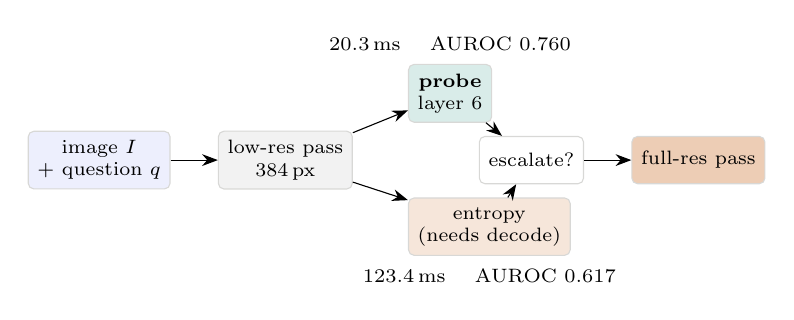
\begin{tikzpicture}[
  box/.style={draw=gwelgrid,rounded corners=2pt,minimum height=6mm,font=\scriptsize,align=center},
  >={Stealth[length=2mm]}, node distance=3mm]
\node[box,fill=gwelblue!8] (img) {image $I$\\+ question $q$};
\node[box,fill=gray!10,right=6mm of img] (cheap) {low-res pass\\$384$\,px};
\node[box,fill=gwelteal!15,above right=1mm and 7mm of cheap] (probe) {\textbf{probe}\\layer 6};
\node[box,fill=gwelorange!15,below right=1mm and 7mm of cheap] (ent) {entropy\\(needs decode)};
\node[box,right=16mm of cheap] (dec) {escalate?};
\node[box,fill=gwelorange!30,right=6mm of dec] (full) {full-res pass};
\draw[->] (img) -- (cheap);
\draw[->] (cheap) -- (probe);
\draw[->] (cheap) -- (ent);
\draw[->] (probe) -- (dec);
\draw[->,dashed] (ent) -- (dec);
\draw[->] (dec) -- (full);
\node[font=\scriptsize,below=0.5mm of ent,text width=3.2cm,align=center]
  {$123.4$\,ms \quad AUROC $0.617$};
\node[font=\scriptsize,above=0.5mm of probe,text width=3.2cm,align=center]
  {$20.3$\,ms \quad AUROC $0.760$};
\end{tikzpicture}
\caption{Two allocation signals read from the same low-resolution pass. Output
entropy requires the pass to complete and generate; the probe reads the
residual stream at layer 6 of 32 and needs no decode.}
\label{fig:pipeline}
\end{figure}

\section{Confidence answers the wrong question}

Mean token entropy over the generated answer predicts $Q_1$ well and $Q_2$
poorly. Table~\ref{tab:targets} reports AUROC on held-out folds, $n=1000$
overall and $n=617$ for $Q_2$.

\begin{table}[t]
\centering\small
\begin{tabular}{lcc}
\toprule
target & output entropy & pre-generation probe \\
\midrule
$Q_1$ correct        & $0.758$ & $0.822$ \\
$Q_2$ escalation helps & $0.617$ & $\mathbf{0.760}$ \\
$Q_3$ answerable     & $0.539$ & $0.681$ \\
\bottomrule
\end{tabular}
\caption{AUROC by target. Entropy is scored with the sign that favours it;
read with the $Q_1$ sign it scores $0.372$ on $Q_2$, because the sign flips
between the two questions.}
\label{tab:targets}
\end{table}

The sign flip is the mechanism. A \emph{confident} wrong answer is a knowledge
failure that more pixels do not fix; an \emph{uncertain} wrong answer is often
a perception failure that they do. Splitting the $617$ failures at their median
entropy, escalation recovers $25\%$ of confident failures and $42\%$ of
uncertain ones.

The two effects reinforce for a policy. Writing the net benefit of escalating as
\begin{equation}
G = \mathbf{1}[\lnot y_{\text{cheap}} \wedge y_{\text{full}}]
  - \mathbf{1}[y_{\text{cheap}} \wedge \lnot y_{\text{full}}],
\end{equation}
$\mathbb{E}[G]$ rises monotonically across entropy quintiles, from $+5\%$ to
$+41.5\%$ (Fig.~\ref{fig:quintiles}). Escalation is worth eight times more in
the top quintile than the bottom.

\begin{figure}[t]
\centering
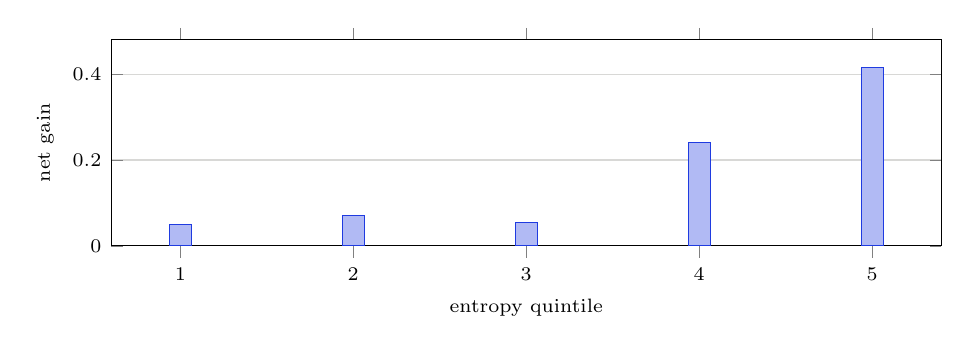
\begin{tikzpicture}
\begin{axis}[
  width=\columnwidth, height=4.2cm,
  ybar, bar width=8pt,
  xlabel={entropy quintile}, ylabel={net gain},
  ymin=0, ymax=0.48, yticklabel={\pgfmathprintnumber{\tick}},
  xtick={1,2,3,4,5}, tick label style={font=\scriptsize},
  label style={font=\scriptsize}, ymajorgrids, grid style={gwelgrid},
]
\addplot[fill=gwelblue!35,draw=gwelblue] coordinates {(1,0.050)(2,0.070)(3,0.055)(4,0.240)(5,0.415)};
\end{axis}
\end{tikzpicture}
\caption{Net benefit of escalating, by entropy quintile ($n=1000$, $200$ per
bin). AUROC of entropy for predicting net benefit is $0.734$.}
\label{fig:quintiles}
\end{figure}

Escalation is also not monotone: $4.1\%$ of queries are answered correctly at
$384$\,px and wrongly at full resolution. No surveyed method models this risk.

\section{A pre-generation probe}
\label{sec:probe}

Following~\cite{lugoloobi,cencerrado}, we read the residual stream
$h^{(\ell)} \in \mathbb{R}^{d}$ at the last prompt position (after the instruction, before any token is generated) and fit the difference-of-means
direction
\begin{equation}
w^{(\ell)} = \mu^{(\ell)}_{+} - \mu^{(\ell)}_{-},
\qquad
s(h) = \frac{(h - \bar\mu^{(\ell)})^\top w^{(\ell)}}{\lVert w^{(\ell)} \rVert},
\label{eq:probe}
\end{equation}
where $\mu_{\pm}$ are class centroids and $\bar\mu$ their midpoint.
Eq.~\ref{eq:probe} is deliberately linear: the question is whether the signal is
linearly accessible, not how well a classifier can be tuned. Stated that way it
is a framing rather than a defence, so we measured what capacity buys
(Table~\ref{tab:family}).

\begin{table}[t]
\centering\small
\setlength{\tabcolsep}{4pt}
\begin{tabular}{lcc}
\toprule
probe family & pooled mixture & within DocVQA \\
\midrule
difference of means & $\mathbf{0.749}$ & $0.576$ \\
logistic & $0.679$ & $0.570$ \\
random Fourier features & $0.699$ & $0.596$ \\
shrunk centroid (LDA) & $0.701$ & $0.579$ \\
\midrule
output entropy & $0.735$ & $\mathbf{0.656}$ \\
\bottomrule
\end{tabular}
\caption{AUROC on the joint escalation target, $20$ resampled folds, layer 6.
Random Fourier features give a smooth non-linear boundary without a bespoke
architecture; the shrunk centroid is the covariance correction the plain
difference of means omits.}
\label{tab:family}
\end{table}

Two things follow, and both are load-bearing. On the mixture the two-centroid
difference \emph{beats} every fitted alternative by $0.048$ or more, so the
paper's probe is not an undertrained stand-in for something better; fitting
parameters on $700$ examples in $960$ dimensions costs more than it recovers.
And within a domain no family closes the gap to output entropy: the best of the
four reaches $0.596$ against entropy's $0.656\ [0.645, 0.666]$. \textbf{The
within-domain negative is a property of the representation, not of linear
models}, which is the objection this table exists to answer. It remains one
family of non-linearities rather than a proof, but it is the family a reviewer
would reach for first. Fitting is a single
pass over cached activations, and the resulting score is the one consumed by the
decision node of Fig.~\ref{fig:pipeline}.

\paragraph{Depth.} Fig.~\ref{fig:layers} sweeps $\ell$. The signal is absent at
$\ell=0$ by construction, the last prompt token is textual and has attended to nothing, and reaches its ceiling by $\ell=3$. Bootstrapped, layer 6 gives
$0.760\ [0.668, 0.849]$ and layer 23 gives $0.760\ [0.652, 0.853]$:
indistinguishable.

\begin{figure}[t]
\centering
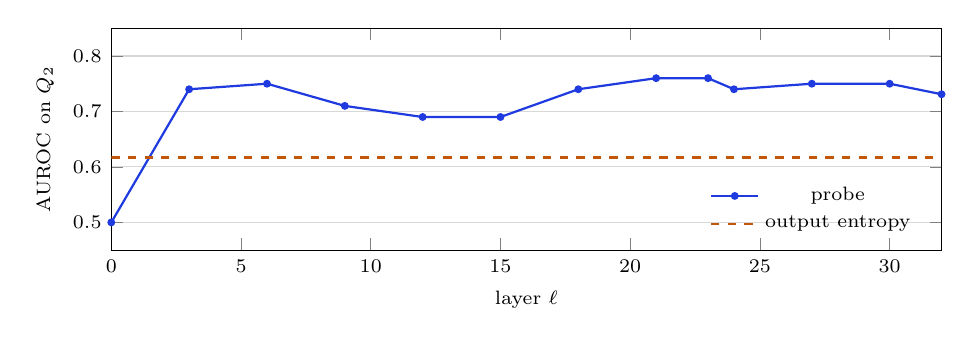
\begin{tikzpicture}
\begin{axis}[
  width=\columnwidth, height=4.4cm,
  xlabel={layer $\ell$}, ylabel={AUROC on $Q_2$},
  xmin=0,xmax=32, ymin=0.45, ymax=0.85,
  tick label style={font=\scriptsize}, label style={font=\scriptsize},
  legend style={font=\scriptsize,at={(0.98,0.03)},anchor=south east,draw=none,fill=none},
  ymajorgrids, grid style={gwelgrid},
]
\addplot[thick,gwelblue,mark=*,mark size=1pt] coordinates {
(0,0.500)(3,0.740)(6,0.750)(9,0.710)(12,0.690)(15,0.690)(18,0.740)
(21,0.760)(23,0.760)(24,0.740)(27,0.750)(30,0.750)(32,0.731)};
\addlegendentry{probe}
\addplot[thick,gwelorange,dashed,no marks] coordinates {(0,0.617)(32,0.617)};
\addlegendentry{output entropy}
\end{axis}
\end{tikzpicture}
\caption{Probe AUROC on $Q_2$ against depth. The ceiling is reached by layer 3
and never improves, so the escalation decision can be made after one sixth of
the language model.}
\label{fig:layers}
\end{figure}

\paragraph{Cost.} Decomposing one pass with CUDA synchronisation around each
component, a $384$\,px pass costs $11.0$\,ms in the vision encoder, $48.1$\,ms
in prefill and $67.8$\,ms in decode. Reading at layer $\ell$ needs the encoder
plus a fraction of prefill,
\begin{equation}
t_{\text{probe}}(\ell) = t_{\text{enc}} + t_{\text{proj}} + \tfrac{\ell}{L}\,t_{\text{prefill}},
\label{eq:probecost}
\end{equation}
giving $20.3$\,ms at $\ell=6$ against $123.4$\,ms for a complete pass.

That ratio is \emph{not} the saving, and it is worth being explicit about why.
Entropy requires the cheap pass to finish, but so does answering, whenever the
policy decides \emph{not} to escalate. The probe therefore saves only on
escalated queries, where the remainder of the cheap pass is abandoned. With
escalation rate $\rho$ and full-resolution cost $t_{\text{full}}$,
\begin{align}
C_{\text{entropy}} &= t_{\text{cheap}} + \rho\, t_{\text{full}},\\
C_{\text{probe}}   &= (1-\rho)\,t_{\text{cheap}} + \rho\,\bigl(t_{\text{probe}} + t_{\text{full}}\bigr).
\label{eq:policycost}
\end{align}
At our observed $\rho \approx 0.30$, Eq.~\ref{eq:policycost} gives $185.3$\,ms
against $154.3$\,ms: a $17\%$ saving, rising to $31\%$ if every query escalates
and falling to $7\%$ at $\rho=0.10$. The probe is cheaper, but by a sixth, not
by the $6\times$ that comparing $t_{\text{probe}}$ from Eq.~\ref{eq:probecost}
against a full pass would suggest. We state this explicitly because the
read-cost ratio is the number an efficiency paper is tempted to report.

\subsection{A better ranking is not a better policy}
\label{sec:policy}

AUROC says a signal orders queries well; it does not say a policy built on it
serves better answers per unit of compute. Building both policies at matched
escalation rates and charging them by Eq.~\ref{eq:policycost} exposes a trap.

A probe trained on $Q_2$ (the \emph{conditional} target, defined only on queries the cheap pass failed) produces a policy that is $8.5$ accuracy points
\emph{worse} than the entropy threshold it beat on AUROC
($-0.085\ [-0.130,-0.040]$, paired). The reason is that a deployed policy must
decide on every query, not only on failures, and the quantity it needs is the
joint event $G$: escalation helps only when the cheap pass would fail
\emph{and} full resolution would succeed. Entropy predicts $G$ at $0.751$
because both factors rise with it. The $Q_2$-trained probe predicts $G$ at
$0.259$, far below chance, because it never saw a successful cheap pass.

Retraining the same probe on $G$ fixes it (Table~\ref{tab:policy}).

\begin{table}[t]
\centering\small
\begin{tabular}{lccc}
\toprule
policy (escalating $30\%$) & accuracy & latency & AUROC on $G$ \\
\midrule
always cheap        & $0.385$ & $123.4$ & n/a \\
entropy threshold   & $0.480$ & $182.2$ & $0.751$ \\
probe on $Q_2$      & $0.395$ & $151.7$ & $0.259$ \\
\textbf{probe on $G$} & $\mathbf{0.510}$ & $\mathbf{154.3}$ & $\mathbf{0.761}$ \\
always full         & $0.530$ & $206.0$ & n/a \\
oracle              & $0.580$ & $139.6$ & n/a \\
\bottomrule
\end{tabular}
\caption{End-to-end policy comparison on the held-out fold, latency in
milliseconds. Against the entropy threshold, the joint-target probe differs in
accuracy by $+0.030\ [-0.005, 0.070]$, indistinguishable, and in latency by
$-27.8\ [-40.7, -15.0]$\,ms, a significant $15\%$ saving.}
\label{tab:policy}
\end{table}

And the $Q_2$ row is the more useful result: a probe can beat a baseline on a
conditional target and lose decisively as a policy. Papers that report ranking
quality without building the policy risk exactly this.

\paragraph{Asking the model directly is worse than reading its uncertainty.}
The escalation mechanism published systems train is a self-report: shown a
downsampled image, the model states whether it needs the full-resolution one.
We cannot reproduce VisionThink's GRPO at sub-1B, that is the premise of this work, but we can implement its \emph{mechanism} without the training, and ask
what the untrained version is worth. Two phrasings were tried, both eliciting a
one-word judgement (Table~\ref{tab:baseline}).

\begin{table}[t]
\centering\small
\begin{tabular}{lccc}
\toprule
policy & escalates & accuracy & latency \\
\midrule
always cheap              & $0\%$  & $0.385$ & $123.4$ \\
self-report, ``ANSWER or ZOOM''  & $7\%$  & $0.385$ & $137.9$ \\
self-report, ``detailed enough?'' & $22\%$ & $0.405$ & $169.8$ \\
entropy threshold         & $20\%$ & $0.465$ & $164.7$ \\
\textbf{probe}            & $20\%$ & $\mathbf{0.475}$ & $\mathbf{144.0}$ \\
always full               & $100\%$& $0.530$ & $206.0$ \\
\bottomrule
\end{tabular}
\caption{Untrained self-report against uncertainty-based routing, $200$
held-out examples, latency in milliseconds. Against the stronger self-report
the probe is $+0.070\ [0.020, 0.120]$ more accurate and $25.8\ [11.9, 39.2]$\,ms
cheaper, both paired and both significant.}
\label{tab:baseline}
\end{table}

The first phrasing escalates $7\%$ of queries and recovers nothing: its accuracy
is exactly that of never escalating, so the compute is pure waste. The second
escalates $22\%$ and buys two accuracy points, where routing on entropy at the
same rate buys eight and routing on the probe buys nine at lower cost. The
self-report is not merely weaker; it escalates as often as the alternatives and
selects the wrong queries.

This bounds what the untrained mechanism delivers and, read the other way,
quantifies what the training in~\cite{visionthink,adaptvision,awares} is buying.
It is not a comparison against those systems, which would require reproducing
their training at a scale where it is not affordable.

\paragraph{The whole frontier, not one operating point.} A single escalation
rate flatters or damns arbitrarily. Sweeping it (Fig.~\ref{fig:frontier}) gives
a cleaner statement: on this fold every entropy operating point is dominated.
Of the fourteen policies evaluated, six lie on the accuracy--cost Pareto front,
four of them probe-based and none entropy-based.

At matched accuracy the saving is $12\%$ at $0.46$ and $22\%$ at $0.52$. The
$0.52$ point matters most: the probe reaches $0.525$ at $161.5$\,ms where always
running at full resolution reaches $0.530$ at $206.0$\,ms, within half a point of the accuracy ceiling for $78\%$ of its cost, while the entropy policy at the
same accuracy costs $206.9$\,ms, marginally \emph{more} than simply always
escalating.

\begin{figure}[t]
\centering
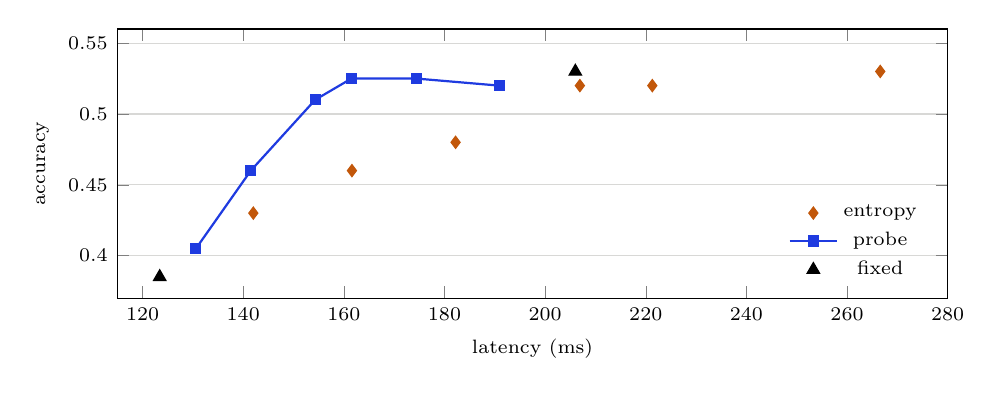
\begin{tikzpicture}
\begin{axis}[
  width=\columnwidth, height=5cm,
  xlabel={latency (ms)}, ylabel={accuracy},
  xmin=115, xmax=280, ymin=0.37, ymax=0.56,
  tick label style={font=\scriptsize}, label style={font=\scriptsize},
  legend style={font=\scriptsize,at={(0.98,0.03)},anchor=south east,draw=none,fill=none},
  ymajorgrids, grid style={gwelgrid},
]
\addplot[only marks,mark=diamond*,mark size=2.2pt,gwelorange] coordinates {
(142.0,0.430)(161.6,0.460)(182.2,0.480)(206.9,0.520)(221.3,0.520)(266.6,0.530)};
\addlegendentry{entropy}
\addplot[thick,gwelblue,mark=square*,mark size=1.6pt] coordinates {
(130.6,0.405)(141.5,0.460)(154.3,0.510)(161.5,0.525)(174.4,0.525)(190.9,0.520)};
\addlegendentry{probe}
\addplot[only marks,mark=triangle*,mark size=2.6pt,black] coordinates {(123.4,0.385)(206.0,0.530)};
\addlegendentry{fixed}
\end{axis}
\end{tikzpicture}
\caption{Accuracy against latency as the escalation rate sweeps from $10\%$ to
$70\%$, on the reported fold. Four probe points lie on the Pareto front,
together with the two fixed policies at its ends. Fig.~\ref{fig:resplit} tests
how much of this survives resplitting.}
\label{fig:frontier}
\end{figure}

\paragraph{How much of that is the fold?} Universal dominance is a statement
about six points on $200$ test examples, and this project has been burned once
already by a conclusion drawn at that scale. We therefore refit everything
downstream of the split (probe direction, thresholds, calibration) on $200$
stratified resplits.

The universal claim does not survive: all seven entropy operating points are
dominated in only $52\%$ of splits. What survives is stronger than that number
suggests. On average $0.83$ of seven entropy points escape domination, and when
one does it wins by a median of $0.010$ accuracy, two queries out of two hundred, with $85\%$ of survivors winning by $0.02$ or less. Meanwhile the
probe holds $90\%$ of the Pareto front, and at matched accuracy it is cheaper
in $200$ of $200$ splits, by a median of $27.8\%$ (Fig.~\ref{fig:resplit}).

\begin{figure}[t]
\centering
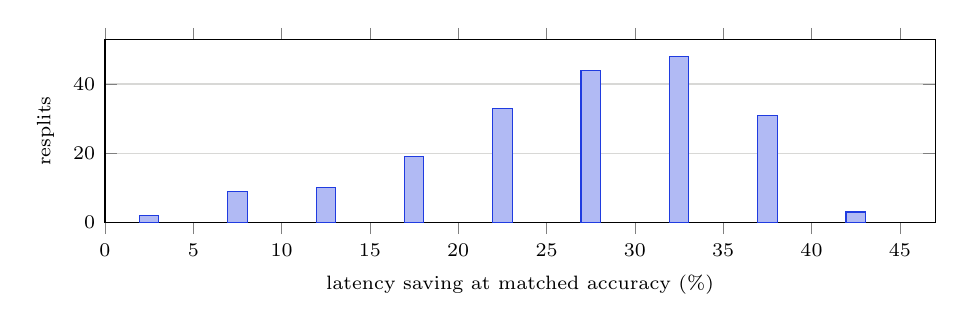
\begin{tikzpicture}
\begin{axis}[
  width=\columnwidth, height=3.9cm,
  ybar, bar width=7pt,
  xlabel={latency saving at matched accuracy (\%)}, ylabel={resplits},
  xmin=0, xmax=47, ymin=0,
  tick label style={font=\scriptsize}, label style={font=\scriptsize},
  ymajorgrids, grid style={gwelgrid},
]
\addplot[fill=gwelblue!35,draw=gwelblue] coordinates {
(2.5,2)(7.5,9)(12.5,10)(17.5,19)(22.5,33)(27.5,44)(32.5,48)(37.5,31)(42.5,3)};
\end{axis}
\end{tikzpicture}
\caption{The probe's latency saving over entropy at matched accuracy, across
$200$ stratified resplits. The distribution is entirely positive; the
single-fold figure of $12\text{--}22\%$ quoted above is a conservative corner of
it.}
\label{fig:resplit}
\end{figure}

The honest summary is that the direction of the effect is robust and its
universality is not. We report the distribution rather than the fold because the
fold is what a single split of $1000$ examples can support.

\paragraph{A better ranking, again, and again no better policy.} Since our own
numbers say the ceiling is the signal, we tried to improve the signal. Entropy
and the probe are complementary: a logistic combination of the two reaches
$0.805$ on the joint target, against $0.751$ and $0.761$ alone, a gain of
$+0.054\ [-0.010, +0.120]$.

As a policy it is strictly worse than the probe alone ($0.505$ accuracy at $181.1$\,ms, against $0.510$ at $154.3$\,ms) because reading entropy requires
finishing the cheap pass, which is precisely the cost the probe existed to
avoid. The best ranking and the best policy are different objects here, and the
second time we observed this it was not a mistake but a structural feature: a
signal's value to a policy is bounded by what it costs to obtain.

\paragraph{How far from the oracle?} Not close, and the shape of the gap is
itself informative. The oracle escalates only $20\%$ of traffic and is
simultaneously more accurate \emph{and} cheaper than always running at full
resolution ($0.580$ at $139.6$\,ms against $0.530$ at $206.0$\,ms). Measured
against the always-cheap baseline, the joint-target probe closes $64\%$ of the
accuracy gap but \emph{increases} cost, where the oracle decreases it. No
policy we build moves along the direction the oracle occupies.

This is the strongest evidence in the paper that the ceiling is the signal
rather than the policy, and it agrees with what the routing literature reports
for text: NVIDIA's prefill-activation router closes $45.6\%$ of its oracle
gap~\cite{llmrouter}, and \cite{lugoloobi} conclude that routing effectiveness
is limited by the reliability of the success estimates, not by the routing rule.

\paragraph{The direction is not domain-general.} Training on detail-limited
datasets (DocVQA, V*Bench) and testing on knowledge-limited ones (VQAv2) gives
$0.422$; the reverse gives $0.366$. Both fall \emph{below} chance: the direction
inverts rather than degrading. The $0.760$ result holds only because the
training fold spans all four datasets. ``Would more pixels help'' is not one
internal quantity but at least two (one for answers present but unreadable, one for answers absent) represented along opposing axes.

\section{What the probe is actually reading}
\label{sec:confound}

A cost measurement, not a literature review, exposed this. Pricing escalation
per example rather than per configuration showed the probe systematically
escalating \emph{larger} images than entropy does, $1.19$ to $1.33\times$ the
visual tokens at matched rate. That is worth explaining, and the explanation
undermines the result above.

\paragraph{The flat escalation price was wrong.} Our profiling image had a
longest side below $1536$\,px, so the processor capped it and the
``full-resolution'' pass spent $320$ visual tokens. On the pilot, \crop{}-free
full passes average $424$ tokens and exceed the $768$ configuration on $44\%$ of
examples. Latency is affine in token count ($100.9 + 0.326\,v$\,ms, worst residual $1.7$\,ms over four profiled configurations) so the honest per-example
price is $238.9$\,ms against the $206.0$ we charged, $16\%$ higher. This is the
third measurement error of the same family we have found, after processor
upscaling and patch-grid quantisation, and all three come from a configuration
name not determining a cost.

Under honest costing the probe's saving over entropy shrinks from
$-27.8\ [-40.7,-15.0]$\,ms to $-11.8\ [-27.2,+5.0]$\,ms at a $30\%$ escalation
rate: no longer distinguishable from zero. It survives at $20\%$ and $40\%$.

\paragraph{Why a better signal picks dearer escalations.} The queries more
pixels help are the queries with more pixels to add. A signal that ranks
escalation value therefore also selects the expensive tail, and ranking quality
partly cancels against cost saving. This is a fourth way a better signal fails a
policy, and unlike the first three it is invisible unless cost is measured per
query rather than per configuration.

\paragraph{And the correlation runs deeper than cost.} If image size predicts
escalation value, it is a routing signal in its own right, and a free one, read
from the file header before any model runs. Table~\ref{tab:confound} scores it
against the two signals the paper has been comparing.

\begin{table}[t]
\centering\small
\setlength{\tabcolsep}{4pt}
\begin{tabular}{lcc}
\toprule
signal & pooled & within one dataset \\
\midrule
image size (free) & $0.748$ & $0.534$ \\
output entropy    & $0.751$ & $\mathbf{0.664}$ \\
pre-generation probe & $\mathbf{0.761}$ & $0.519$ \\
\bottomrule
\end{tabular}
\caption{Predicting the joint escalation gain. Pooled is the held-out fold of
the four-dataset mixture, $n=200$. Within-dataset trains and tests the probe
inside a single dataset over $40$ resamples, weighted by dataset size.}
\label{tab:confound}
\end{table}

The probe's margin over a feature costing nothing is $+0.013$. And the
within-dataset column is the result (Fig.~\ref{fig:confound}): with the
between-domain axis removed the probe is at chance in every dataset (DocVQA
$0.502\ [0.483, 0.521]$, VQAv2 $0.468\ [0.422, 0.513]$) while output entropy
retains $0.664$. Each of these fits sees only $210$ training examples, which is
a confound of its own; \S\ref{sec:singledomain} removes it with a pilot built
for the purpose.

\begin{figure}[t]
\centering
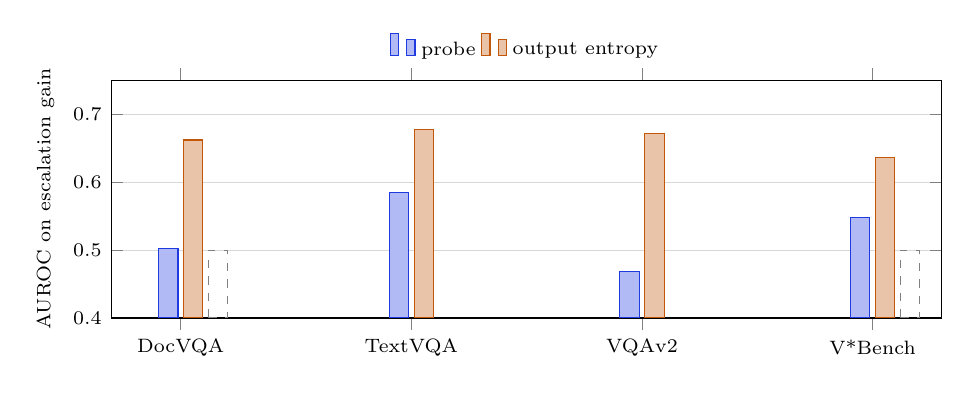
\begin{tikzpicture}
\begin{axis}[
  width=\columnwidth, height=4.6cm,
  ybar, bar width=7pt,
  symbolic x coords={DocVQA,TextVQA,VQAv2,V*Bench},
  xtick=data, ymin=0.40, ymax=0.75,
  ylabel={AUROC on escalation gain},
  tick label style={font=\scriptsize}, label style={font=\scriptsize},
  legend style={font=\scriptsize,at={(0.5,1.04)},anchor=south,legend columns=2,draw=none,fill=none},
  ymajorgrids, grid style={gwelgrid},
]
\addplot[fill=gwelblue!35,draw=gwelblue] coordinates {
(DocVQA,0.502)(TextVQA,0.585)(VQAv2,0.468)(V*Bench,0.548)};
\addlegendentry{probe}
\addplot[fill=gwelorange!35,draw=gwelorange] coordinates {
(DocVQA,0.662)(TextVQA,0.677)(VQAv2,0.671)(V*Bench,0.636)};
\addlegendentry{output entropy}
\addplot[gray,dashed,no marks,forget plot] coordinates {(DocVQA,0.5)(V*Bench,0.5)};
\end{axis}
\end{tikzpicture}
\caption{Within a single dataset, trained and tested inside it. The dashed line
is chance. The probe's pooled advantage does not survive removal of the
between-domain axis; entropy's largely does.}
\label{fig:confound}
\end{figure}

\paragraph{What the disagreement looks like.} The statistics above say the probe
tracks image size; the queries say what that means. Ranking the held-out fold by
each signal and taking the largest rank disagreements, the two sets are almost
disjoint by dataset (Table~\ref{tab:disagree}).

\begin{table}[t]
\centering\small
\setlength{\tabcolsep}{4pt}
\begin{tabular}{lcccc}
\toprule
& DocVQA & TextVQA & VQAv2 & V*Bench \\
\midrule
test fold & $30\%$ & $25\%$ & $30\%$ & $15\%$ \\
probe favours & $\mathbf{50\%}$ & $36\%$ & $12\%$ & $2\%$ \\
entropy favours & $\mathbf{0\%}$ & $28\%$ & $46\%$ & $26\%$ \\
\bottomrule
\end{tabular}
\caption{Dataset composition of the $50$ queries where each signal most wants to
escalate relative to the other. Not one of the queries entropy prefers is a
DocVQA page.}
\label{tab:disagree}
\end{table}

\textbf{The disagreement between the two signals predicts which dataset a query
came from at AUROC $0.738$}, which is most of what either signal achieves on the
escalation target itself. Where they differ, they differ about what kind of
image it is.

The individual queries are unambiguous. The four the probe most wants to
escalate are all DocVQA, all $448\text{--}640$ visual tokens at full resolution,
and all have $G = 0$: ``What is written in big letters on the top right?'' is
answered \emph{correctly} at $384$\,px and the escalation changes nothing. The
four entropy most wants to escalate are all VQAv2 photographs at $320$ tokens,
all wrong at both resolutions, questions like ``What is tucked behind the
lamp?'' where the model is genuinely lost and more pixels do not help.

Read charitably this is the probe doing something reasonable, since documents do
repair more often on average. Read as a routing signal it is a category
detector: it escalates a correct answer on a large page and declines a hopeless
one on a small photograph, and neither decision used anything about the query.

\paragraph{The text-probe literature saw this coming, and evaluates
accordingly.} Having found it, we went back to check whether the work we build
on is exposed to the same thing. It is not, and one of them names the mechanism.
Moreno Cencerrado et al.~\cite{cencerrado} train and test their correctness
direction \emph{within} each dataset and report cross-dataset transfer
separately, and observe that for some sources ``the learned direction captures
dataset-specific cues correlated with correctness rather than correctness
itself''. Lugoloobi et al.~\cite{lugoloobi} likewise average AUROC over their
benchmarks rather than pooling examples across them. Neither pools; we did.

Two of their observations also validate the test we use here. Cencerrado et al.
report that probe performance on GSM8K ``plateaus near random chance regardless
of dataset size'', distinguishing an absent signal from an under-sampled one by
exactly the learning-curve argument, and they find a non-linear classifier on
external embeddings generalising \emph{worse} than a linear probe on internal
states, the opposite of what a capacity explanation would predict. The
correction here is therefore to our evaluation protocol, not to their finding.

\paragraph{This explains a result we had already reported and misread.} We
found earlier that the probe's direction inverts across domains (trained on detail-limited data and tested on knowledge-limited data it scores $0.422$, and the reverse $0.366$, both below chance) and read it as a transfer limitation
calling for a domain-representative calibration set. The correct reading is
stronger: a direction that carries no within-domain signal and inverts between
domains is a domain classifier, and its pooled AUROC measures how separable the
mixture is, not how well the model knows its own needs. Both facts were in our
data; only the second explains them.

\subsection{A single-domain pilot, and what it settles}
\label{sec:singledomain}

The within-domain fit above gets $210$ training examples where the pooled fit
gets $600$, so part of the collapse could be sample size rather than absent
signal. We said so, and then collected the pilot that decides it: $1200$ DocVQA
pages, enough to fit and test inside one domain.

The decisive form is a learning curve. If the probe were merely starved, AUROC
would climb toward the pooled figure as training data grows. Neither extreme is
what happens (Fig.~\ref{fig:curve}).

\begin{figure}[t]
\centering
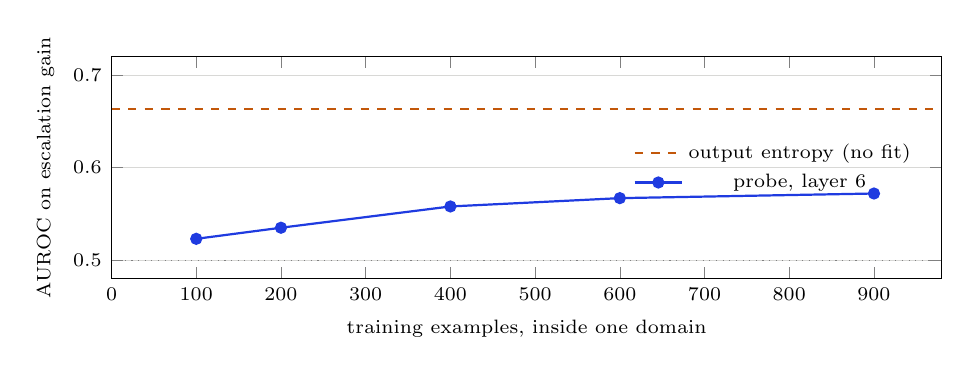
\begin{tikzpicture}
\begin{axis}[
  width=\columnwidth, height=4.4cm,
  xlabel={training examples, inside one domain}, ylabel={AUROC on escalation gain},
  xmin=0, xmax=980, ymin=0.48, ymax=0.72,
  tick label style={font=\scriptsize}, label style={font=\scriptsize},
  legend style={font=\scriptsize,at={(0.98,0.5)},anchor=east,draw=none,fill=none},
  ymajorgrids, grid style={gwelgrid},
]
\addplot[thick,gwelorange,dashed,no marks] coordinates {(0,0.663)(980,0.663)};
\addlegendentry{output entropy (no fit)}
\addplot[thick,gwelblue,mark=*,mark size=1.8pt] coordinates {
(100,0.523)(200,0.535)(400,0.558)(600,0.567)(900,0.572)};
\addlegendentry{probe, layer 6}
\addplot[gray,dotted,no marks] coordinates {(0,0.5)(980,0.5)};
\end{axis}
\end{tikzpicture}
\caption{Probe AUROC inside DocVQA against training size, $30$ resamples with a
fixed $300$-example held-out set. The dotted line is chance. More data helps and
does not close the gap: at $900$ examples, more than the pooled fit that
produced $0.761$, the probe reaches $0.572$.}
\label{fig:curve}
\end{figure}

The probe does improve, by $+0.050$ as training data grows ninefold, so the
collapse is not purely starvation. But it plateaus far below output entropy,
which is fitted on nothing. \textbf{The signal is genuinely weaker inside a
domain than the pooled figure suggests}, and the confound conclusion stands in
this corrected form rather than as ``at chance''.

\paragraph{And the depth that works does not transfer either.} We selected layer
6 because AUROC saturates there on the mixture, and the entire read-cost
argument of \S\ref{sec:probe} rests on stopping a sixth of the way through the
language model. Inside one domain the signal keeps improving with depth:

\begin{center}\small
\begin{tabular}{lcccccc}
\toprule
layer & 1 & 3 & 6 & 12 & 20 & 32 \\
\midrule
AUROC & $0.531$ & $0.546$ & $0.572$ & $0.579$ & $0.618$ & $\mathbf{0.625}$ \\
\bottomrule
\end{tabular}
\end{center}

\noindent The best depth is the last one. That costs the probe its cheap read:
Eq.~\ref{eq:probecost} gives $20.0$\,ms at $\ell=6$ and $59.1$\,ms at
$\ell=32$, so the saving per escalated query falls from $106.9$ to $67.8$\,ms.

Two things are worth noting about that residual $67.8$\,ms. It is exactly the
decode time, because a full-prefill probe still skips generation, and it is the
same floor the cache analysis of \S\ref{sec:cost} arrived at from an unrelated
direction. The probe's advantage narrows to one mechanism, stated twice: reading
the model without making it speak.

\paragraph{An independent corroboration of the corrected depth.}
GlimpsePrune~\cite{glimpseprune} reads its learned glimpse token at layer $K =
\tfrac{2}{3}L$, chosen as the point where it has ``aggregated sufficiently clear
importance information'' at a favourable overhead trade-off. That is where our
within-domain sweep becomes informative ($0.618$ at layer $20$ of $32$) and far
from the layer $6$ the mixture selected. Two groups reading different internal
signals for different purposes land on the same region of the network, which is
weak evidence but it points the same way as \S\ref{sec:singledomain}: the
shallow saturation was the artefact, not the deep one.

\paragraph{What survives.} Three things. The mixture result is real and
mixtures are real deployments: a router serving documents and photographs
through one endpoint faces exactly the pooled distribution, and there a free
image-size feature is nearly as good and much cheaper than either signal we
studied. The negative results are untouched, since none of them rests on the
probe working. And the paper's thesis survives inverted: we set out to show that
a better signal is not a better router, and the sharpest instance turns out to
be our own signal, whose advantage was an artefact of the evaluation mixture.

\paragraph{What does not.} The claim that a $500$M VLM encodes its need for more
pixels in a linearly readable direction. On the evidence here it mostly encodes
what kind of image it is looking at, which correlates with that need across a
benchmark mixture and much less within one. \S\ref{sec:singledomain} is the
test we said this needed, run on a corpus built for it, and it does not rescue
the claim: given nine times the training data the direction reaches $0.572$
where the model's own output entropy, fitted on nothing, reaches $0.663$. The
honest statement is that the direction carries some within-domain signal and
less than the cheaper alternative.

\section{The escalation rate is not a free parameter}
\label{sec:rule}

Every policy above picks a rate and thresholds at that quantile. That is a
tuning exercise, and nothing connects the chosen rate to Eq.~\ref{eq:cost}, the
cost function the oracle is already labelled under. Kotte's UCCI~\cite{ucci}
closes the same gap for text cascades (calibrate the signal to a probability, then let the cost model choose the threshold) and its transposition here is
short, but it needs one correction.

\paragraph{The rule.} Escalating $x$ changes expected cost by
\begin{equation}
\Delta J(x) = -\,w_e\,\mathbb{E}[G \mid x] + \lambda_t\,\Delta t,
\label{eq:deltaj}
\end{equation}
so the optimal action is to escalate exactly when
\begin{equation}
\mathbb{E}[G \mid x] \;>\; \tau = \frac{\Delta t}{V},
\qquad V = \frac{w_e}{\lambda_t},
\label{eq:breakeven}
\end{equation}
where $V$ is the only knob: the latency an operator will spend to buy one
additional correct answer, in milliseconds. Following~\cite{clusterroute}, we
state the trade-off in the units of the outcome rather than as a weight per
millisecond, because the latter is not readable across devices. Estimating
$\mathbb{E}[G \mid x]$ from the probe score by isotonic regression (monotone, non-parametric, one pass over cached activations) gives Algorithm~1.

\begin{figure}[t]
\small
\hrule\vspace{2pt}
\textbf{Algorithm 1} Calibrated gain-optimal escalation
\vspace{1pt}\hrule\vspace{3pt}
\begin{tabbing}
xx\=xx\=xx\=\kill
\textbf{fit} \\
1\> read $h^{(\ell)}$ at the last prompt position, $\ell = 6$ \\
2\> $G_i \leftarrow \mathbf{1}[\lnot y^{\text{cheap}}_i \wedge y^{\text{full}}_i]
       - \mathbf{1}[y^{\text{cheap}}_i \wedge \lnot y^{\text{full}}_i]$ \\
3\> $w \leftarrow \mu_+ - \mu_-$ over $\{G_i > 0\}$ vs.\ the rest \\
4\> $s_i \leftarrow (h_i - \bar\mu)^\top w / \lVert w \rVert$ \\
5\> $\hat g \leftarrow 2\,\mathrm{isotonic}\bigl(s,\ (G+1)/2\bigr) - 1$ \\
\textbf{serve} $x$, given $V$ \\
6\> $\Delta t \leftarrow t_{\text{probe}} + t_{\text{full}} - t_{\text{cheap}}$ \\
7\> \textbf{if} $\hat g(s(x)) > \Delta t / V$ \textbf{then} abandon the prefill,
     run full \\
8\> \textbf{else} finish the cheap pass and answer
\end{tabbing}
\vspace{-4pt}\hrule
\end{figure}

\paragraph{Why isotonic, and what actually matters about it.} We take isotonic
regression from~\cite{ucci}, and borrowing a component is how a paper inherits
someone else's assumptions. The settings differ where calibration is sensitive:
their target is a probability with tens of thousands of calibration points, ours
a signed gain with a few hundred. Three families thresholded at the \emph{same}
break-even, so any difference is the calibrator's magnitudes rather than a
different operating point (Table~\ref{tab:calibrator}).

\begin{table}[t]
\centering\small
\setlength{\tabcolsep}{4pt}
\begin{tabular}{lccc}
\toprule
calibrator & AUROC & calib.\ error & accuracy \\
\midrule
isotonic & $0.660$ & $0.059$ & $\mathbf{0.736}$ \\
Platt sigmoid & $\mathbf{0.667}$ & $0.098$ & $0.713$ \\
equal-mass bins & $0.656$ & $\mathbf{0.051}$ & $0.733$ \\
\bottomrule
\end{tabular}
\caption{Calibrator families on $1200$ DocVQA pages, $30$ resamples, all
thresholded at $\tau = 0.243$. Paired against isotonic, Platt loses $0.022\
[-0.026, -0.019]$ accuracy and equal-mass bins differ by $-0.003\ [-0.006,
0.000]$.}
\label{tab:calibrator}
\end{table}

The sigmoid ranks marginally \emph{best} and calibrates worst, at nearly twice
the error, and its policy is significantly less accurate. That is the paper's
recurring pattern arriving in a third place: ranking quality does not transfer,
this time because a rule that thresholds a magnitude is broken by a
miscalibrated magnitude in a way a rank threshold would never notice. A
parametric squash reports gains the operator did not ask for, and the rule
lands somewhere other than the point $V$ specifies.

Equal-mass bins, meanwhile, are indistinguishable from isotonic. \textbf{The
load-bearing property is being non-parametric, not being isotonic}, and we say
so rather than defend a component we happened to inherit. Isotonic remains the
better default because monotonicity is free information that binning discards,
but nothing here rests on it.

\paragraph{When the rule is optimal, and how it relates to UCCI's theorem.}
Eq.~\ref{eq:breakeven} is not a heuristic. Let $s(x)$ be any routing score and
let $\Pi_s$ be the policies measurable with respect to it, which is what a
deployed router is: it sees the score, not the outcome.

\vspace{2pt}
\noindent\textbf{Proposition 1.} \emph{Under the cost of Eq.~\ref{eq:cost} with
$w_e, \lambda_t > 0$, and given the calibrated gain $\hat g(s) = \mathbb{E}[G
\mid s]$, the policy}
\[
\pi^\star(x) = \mathbf{1}\bigl[\hat g(s(x)) > \Delta t / V\bigr],
\qquad V = w_e/\lambda_t,
\]
\emph{minimises expected cost over $\Pi_s$. If $\hat g$ is non-decreasing, it is
a threshold on $s$ itself.}

\vspace{2pt}
\noindent\emph{Proof.} Write $C(\pi) = C_0 + \mathbb{E}\bigl[\pi(x)\,\Delta
J(x)\bigr]$, where $C_0$ is the cost of answering cheap on every query and
$\Delta J$ is Eq.~\ref{eq:deltaj}. The expectation is linear in $\pi$ and the
constraint set is $\pi(x) \in \{0,1\}$, so it is minimised pointwise by
escalating exactly where $\Delta J(x) < 0$. For $\pi \in \Pi_s$ the tower
property gives $\mathbb{E}[\Delta J \mid s] = -w_e\,\mathbb{E}[G \mid s] +
\lambda_t \Delta t$, so the pointwise test becomes $\hat g(s) > \lambda_t \Delta
t / w_e$. Monotone $\hat g$ makes the sublevel set an interval in $s$. $\square$

\vspace{2pt}
Two things follow. Isotonic regression returns a non-decreasing $\hat g$ by
construction, so Algorithm~1 realises $\pi^\star$ whenever the calibration is
accurate, which Fig.~\ref{fig:reliability} measures rather than assumes. And the
relation to Kotte's Theorem~1~\cite{ucci} is exact: under their assumption that
the escalated pass attains a fixed accuracy $\gamma$ independent of which
queries are sent, $\mathbb{E}[G \mid x] = \gamma - (1 - p_{\text{err}}(x))$,
which is increasing in the weak model's error probability, so their rule and
ours coincide. \textbf{The two rules agree exactly when escalation cannot make
things worse, and Table~\ref{tab:rule} is what their difference costs when it
can.}

\paragraph{The break-even is signal-dependent, and that is the probe's second
advantage.} Line 6 differences Eq.~\ref{eq:policycost}. A policy reading entropy
must finish the cheap pass before deciding, so escalation adds the whole
full-resolution pass, $\Delta t = 206.0$\,ms. A policy reading the probe
abandons the cheap pass it never completed, so $\Delta t = 20.3 + 206.0 - 123.4
= 102.9$\,ms, exactly half. At the same operator preference $V$, the probe's
break-even gain is half entropy's: \textbf{a cheaper signal is entitled to
escalate on weaker evidence}, and the saving compounds rather than merely
lowering the bill for a fixed rate.

\paragraph{Calibrating the wrong probability.} UCCI's Theorem~1 assumes the
strong model attains a fixed accuracy on the escalated subset, invariant to
which queries are sent. Under that assumption the escalation value of a query is
determined by the weak model's error probability, so calibrating $P(\text{cheap
wrong})$ suffices. Visual escalation violates it: it is non-monotone, repairing
$21\%$ of queries and \emph{damaging} $4\%$, so the escalated pass is a second
random outcome rather than a fixed accuracy. The quantity to calibrate is the
signed gain, and the difference is not academic (Table~\ref{tab:rule}).

\begin{table}[t]
\centering\small
\begin{tabular}{lcccc}
\toprule
rule & calibration target & escalates & accuracy & latency \\
\midrule
UCCI~\cite{ucci} & $P(\text{cheap wrong})$ & $54\%$ & $0.520$ & $178.5$ \\
\textbf{ours} & $\mathbb{E}[G \mid x]$ & $\mathbf{34\%}$ & $0.520$ & $\mathbf{157.9}$ \\
\bottomrule
\end{tabular}
\caption{Both rules read the same probe score at $V = 800$\,ms per correct
answer and differ only in what they calibrate. Paired, the accuracy difference
is $0.000\ [-0.025, 0.025]$ and the latency difference $-20.6\ [-26.8,
-14.9]$\,ms: the same answers for $59\%$ relatively more compute.}
\label{tab:rule}
\end{table}

The failure is legible. A confidently wrong cheap pass has high error
probability and near-zero expected gain, so UCCI escalates it and the gain rule
does not, the same conditional-versus-joint error of \S\ref{sec:policy},
displaced from the training target to the calibration target. Fitting the gain
directly is well calibrated: binned over the held-out fold, predicted and
realised gain agree to $0.029$ (Fig.~\ref{fig:reliability}), against a
correctness ECE of $0.027$ for the same signal, so the correction costs nothing
in calibration quality.

\begin{figure}[t]
\centering
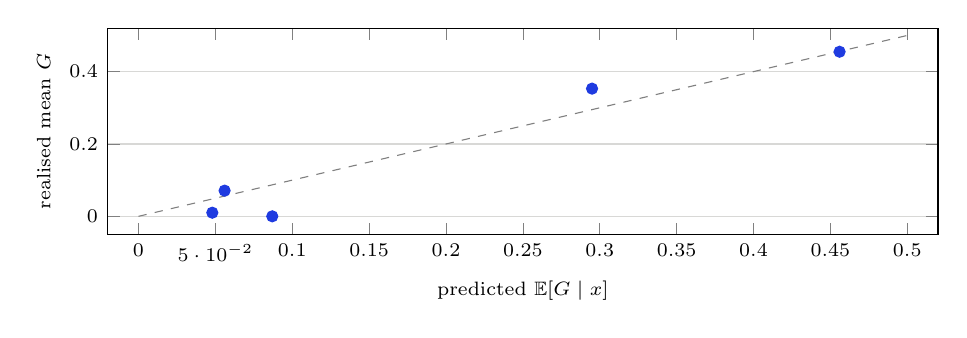
\begin{tikzpicture}
\begin{axis}[
  width=\columnwidth, height=4.2cm,
  xlabel={predicted $\mathbb{E}[G \mid x]$}, ylabel={realised mean $G$},
  xmin=-0.02,xmax=0.52, ymin=-0.05, ymax=0.52,
  tick label style={font=\scriptsize}, label style={font=\scriptsize},
  ymajorgrids, grid style={gwelgrid},
]
\addplot[gray,dashed,no marks] coordinates {(0,0)(0.5,0.5)};
\addplot[only marks,mark=*,mark size=2pt,gwelblue] coordinates {
(0.048,0.010)(0.056,0.071)(0.087,0.000)(0.295,0.353)(0.456,0.455)};
\end{axis}
\end{tikzpicture}
\caption{Reliability of the gain calibration on the held-out fold, binned by
predicted gain. The dashed line is perfect calibration. A rule that thresholds a
\emph{magnitude} is only as good as the magnitude, which a ranking metric would
not detect.}
\label{fig:reliability}
\end{figure}

\paragraph{Does removing the knob cost anything?} It should not, if the rule is
right. Sweeping $V$ over $100$--$3200$\,ms per correct answer places six
operating points on the accuracy--latency plane without any rate ever being
chosen; five of the six are undominated by the tuned sweep of
Fig.~\ref{fig:frontier} evaluated on the same fold (Fig.~\ref{fig:rule}), and
$78\%$ remain undominated across the $200$ resplits. An untuned rule reaches a
tuned frontier, which is the useful form of this result: the rate was never
information, only a stand-in for a preference the operator already has.

\begin{figure}[t]
\centering
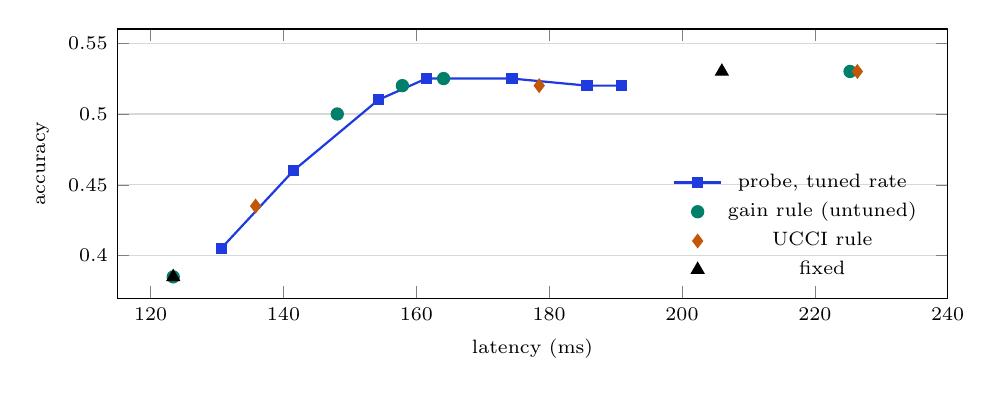
\begin{tikzpicture}
\begin{axis}[
  width=\columnwidth, height=5cm,
  xlabel={latency (ms)}, ylabel={accuracy},
  xmin=115, xmax=240, ymin=0.37, ymax=0.56,
  tick label style={font=\scriptsize}, label style={font=\scriptsize},
  legend style={font=\scriptsize,at={(0.98,0.03)},anchor=south east,draw=none,fill=none},
  ymajorgrids, grid style={gwelgrid},
]
\addplot[thick,gwelblue,mark=square*,mark size=1.6pt] coordinates {
(130.6,0.405)(141.5,0.46)(154.3,0.51)(161.5,0.525)(174.4,0.525)(185.7,0.52)(190.9,0.52)};
\addlegendentry{probe, tuned rate}
\addplot[only marks,mark=*,mark size=2.2pt,gwelteal] coordinates {
(123.4,0.385)(148.1,0.5)(157.9,0.52)(164.1,0.525)(225.3,0.53)};
\addlegendentry{gain rule (untuned)}
\addplot[only marks,mark=diamond*,mark size=2.4pt,gwelorange] coordinates {
(135.8,0.435)(178.5,0.52)(226.4,0.53)};
\addlegendentry{UCCI rule}
\addplot[only marks,mark=triangle*,mark size=2.6pt,black] coordinates {(123.4,0.385)(206.0,0.530)};
\addlegendentry{fixed}
\end{axis}
\end{tikzpicture}
\caption{Untuned decision rules against the tuned sweep. The gain rule tracks
the swept frontier without a rate parameter; the UCCI rule, calibrating
correctness instead, sits inside it and collapses to always-escalate once $V$ is
large.}
\label{fig:rule}
\end{figure}

\paragraph{Where the rule refuses.} At $V \le 200$ the break-even of
Eq.~\ref{eq:breakeven} exceeds any attainable gain and the rule escalates
nothing, returning the always-cheap policy. That is the correct answer, not a
degenerate one: by Eq.~\ref{eq:deltaj} no expected gain on this pilot repays
$102.9$\,ms when a correct answer is worth $200$. A tuned rate cannot express
this, which is the failure mode reported for our earlier threshold tuners, they
discovered ``never escalate'' on one fold and had no way to say whether that was
a preference or an artefact. Where a floor on escalation is required instead,
\cite{recall}'s recall-controlled gates give one that cannot degenerate by
construction.

\subsection{The rule transfers where the signal does not}
\label{sec:transfer}

Every number above uses the probe, which \S\ref{sec:confound} discredits within
a domain. So we re-ran the whole comparison on output entropy, the signal that does work within a domain, fitted and tested inside each dataset over $40$
resamples, with escalation priced per example. If the rule is a property of the
method rather than of the signal, it should survive.

It does, and the confound makes it more useful rather than less. Escalation
value is domain-determined, so a fixed rate is wrong in every domain but the one
it was tuned on. A rule calibrated on the observed gain distribution picks its
own rate wherever it is fitted, from one unchanged operator preference
(Fig.~\ref{fig:transfer}).

\begin{figure}[t]
\centering
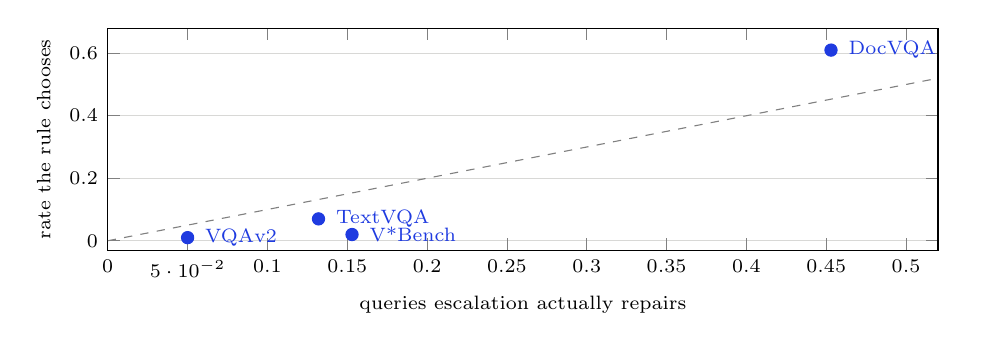
\begin{tikzpicture}
\begin{axis}[
  width=\columnwidth, height=4.4cm,
  xlabel={queries escalation actually repairs}, ylabel={rate the rule chooses},
  xmin=0, xmax=0.52, ymin=-0.03, ymax=0.68,
  xticklabel={\pgfmathprintnumber{\tick}}, yticklabel={\pgfmathprintnumber{\tick}},
  tick label style={font=\scriptsize}, label style={font=\scriptsize},
  ymajorgrids, grid style={gwelgrid},
  nodes near coords, point meta=explicit symbolic,
  every node near coord/.append style={font=\scriptsize,anchor=west,xshift=1mm},
]
\addplot[gray,dashed,no marks] coordinates {(0,0)(0.52,0.52)};
\addplot[only marks,mark=*,mark size=2.2pt,gwelblue] coordinates {
(0.050,0.01)[VQAv2] (0.132,0.07)[TextVQA] (0.153,0.02)[V*Bench] (0.453,0.61)[DocVQA]};
\end{axis}
\end{tikzpicture}
\caption{One value of $V$, applied unchanged to four domains. The rule escalates
$61\%$ of DocVQA and $1\%$ of VQAv2, tracking how much escalation actually
repairs there ($r=0.974$). The dashed line is not a target, escalating every repairable query is not optimal, but it fixes the scale.}
\label{fig:transfer}
\end{figure}

Fixing one policy and applying it to all four domains, weighted by dataset size,
the rule reaches $0.489$ accuracy at $181.6$\,ms where a tuned $30\%$ rate
reaches $0.464$ at $195.1$\,ms: more accurate \emph{and} cheaper. Tuned rates at
$40\%$ and $50\%$ are dominated as well. Only the two lowest tuned rates survive
on the front, at the cautious end where escalating little is right everywhere.

\subsection{How far to escalate, not just whether}
\label{sec:ladder}

Every escalation method we have read is binary: answer from a downsampled image,
or run the full one. Taking the cheapest configuration that answers each query
correctly says that collapses the decision carrying most of the money.

\begin{center}\small
\begin{tabular}{lc}
\toprule
cheapest rung that answers correctly & share \\
\midrule
$384$\,px (no escalation) & $38.3\%$ \\
intermediate rung & $\mathbf{17.7\%}$ \\
full resolution & $5.2\%$ \\
nothing we run & $38.8\%$ \\
\bottomrule
\end{tabular}
\end{center}

\noindent Of the queries escalation can repair, $77\%$ are repaired by the
intermediate rung. A binary policy over-serves three quarters of what it
escalates. The rungs are also not equally efficient: $384 \to 768$ buys $13.3$
points for $79$\,ms ($+1.69$ points per second) where $768 \to$ full buys $3.3$
for $38$\,ms ($+0.86$). The binary jump measures $+1.42$, which is what
averaging a good rung with a poor one gives.

\paragraph{The rule generalises without modification.} Rung $r$ has its own
expected gain over answering cheap and its own extra latency, so
\begin{equation}
r^\star(x) = \arg\max_r \;\bigl(V\,\mathbb{E}[G_r \mid x] - \Delta t_r\bigr),
\label{eq:ladder}
\end{equation}
answering cheap when no rung is positive. Eq.~\ref{eq:ladder} reduces to
Eq.~\ref{eq:breakeven} when there is one rung; the binary policy is the special
case that has deleted the middle of its own ladder. One calibrator per rung is
fitted on the same score, so the additional cost is a second isotonic fit over
cached values.

\begin{figure}[t]
\small
\hrule\vspace{2pt}
\textbf{Algorithm 2} Calibrated ladder escalation
\vspace{1pt}\hrule\vspace{3pt}
\begin{tabbing}
xx\=xx\=xx\=\kill
\textbf{fit}, given rungs $r = 1 \dots R$ in increasing cost \\
1\> $s_i \leftarrow$ any routing score read from the cheap pass \\
2\> \textbf{for} each rung $r$: \\
3\> \> $G^{(r)}_i \leftarrow \mathbf{1}[\lnot y^{\text{cheap}}_i \wedge y^{r}_i]
        - \mathbf{1}[y^{\text{cheap}}_i \wedge \lnot y^{r}_i]$ \\
4\> \> $\hat g_r \leftarrow 2\,\mathrm{isotonic}\bigl(s,\ (G^{(r)}+1)/2\bigr) - 1$ \\
\textbf{serve} $x$, given $V$ \\
5\> $\Delta t_r \leftarrow t_r(x) - t_{\text{cheap}}(x)$ \ \ for each rung \\
6\> $v_r \leftarrow V\,\hat g_r(s(x)) - \Delta t_r$ \\
7\> \textbf{if} $\max_r v_r > 0$ \textbf{then} run rung $\arg\max_r v_r$ \\
8\> \textbf{else} answer from the cheap pass
\end{tabbing}
\vspace{-4pt}\hrule
\end{figure}

Proposition~1 extends without change. Escalating to rung $r$ shifts expected
cost by $\Delta J_r(x) = -w_e\,\mathbb{E}[G_r \mid x] + \lambda_t \Delta t_r$,
the choice is again pointwise because the objective is linear in the selection,
and the best action at $x$ is the rung minimising $\Delta J_r$, or the cheap
pass when every $\Delta J_r$ is non-negative. Multiplying through by $-1/
\lambda_t$ gives Eq.~\ref{eq:ladder}. The binary rule is therefore not a
simplification of the ladder but a \emph{constrained} version of it, forced to
choose between two of the rungs available to it.

\paragraph{It pays where the ladder physically exists, and nowhere else.}
Paired over four domains and four preferences, the ladder is
$-9.6\ [-17.2,-2.6]$\,ms cheaper at $-0.003\ [-0.008,+0.002]$ accuracy:
significantly cheaper, indistinguishable in accuracy. The per-domain breakdown
is the real result (Table~\ref{tab:ladder}).

\begin{table}[t]
\centering\small
\setlength{\tabcolsep}{4pt}
\begin{tabular}{lccc}
\toprule
 & top rung exists & accuracy & latency \\
\midrule
DocVQA  & $98\%$ & $+0.003$ & $\mathbf{-35.1}$ \\
V*Bench & $98\%$ & $-0.008$ & $-3.5$ \\
TextVQA & $0\%$  & $-0.006$ & $+1.2$ \\
VQAv2   & $0\%$  & $-0.002$ & $-0.8$ \\
\bottomrule
\end{tabular}
\caption{Ladder minus binary, averaged over four operator preferences, latency
in milliseconds. ``Top rung exists'' is the share of images on which the
full-resolution pass spends more visual tokens than the intermediate one.}
\label{tab:ladder}
\end{table}

On DocVQA the ladder saves $35$\,ms at no accuracy cost. On TextVQA and VQAv2 it
does nothing, correctly, because for those datasets there is no top rung to
find.

\paragraph{A configuration name does not determine a configuration.} That last
column is a measurement fact worth stating on its own. The processor caps its
target at the input's longest side, so on a small image the ``full-resolution''
pass \emph{is} the intermediate pass: identical token count, identical cost,
identical output. This holds for $100\%$ of TextVQA and VQAv2 and $2\%$ of the
other two, $56\%$ of the pilot. The escalation this paper studies is a real
escalation for half its data.

This is the fourth error of the same family we have found, after processor
upscaling, patch-grid quantisation, and the flat escalation price of
\S\ref{sec:confound}. All four come from treating a configuration label as a
cost or a capability. The general form of the lesson: in adaptive-resolution
work, verify that the configurations differ \emph{on the data}, not in the
config file.

\paragraph{A ladder built on measured rungs, and where it stops.} The mixture
cannot price the second and third rungs, because for over half of it they are
the same configuration. So we collected a single-domain pilot designed against
that: $1200$ DocVQA pages, with rungs chosen by measuring SmolVLM's patch-grid
buckets ($64$, $320$, $640$ and $1088$ visual tokens) rather than by picking
round pixel sizes. Every rung is strictly dearer than the one below it on
$95\text{--}100\%$ of images, and latency is affine in tokens at
$205.0 + 0.415\,v$\,ms with a worst residual of $20.2$\,ms.

The result is a saturation point, and it arrives early
(Table~\ref{tab:saturation}).

\begin{table}[t]
\centering\small
\setlength{\tabcolsep}{4pt}
\begin{tabular}{lccc}
\toprule
step & net gain [95\% CI] & cost & points/s \\
\midrule
$64 \to 320$   & $+0.383\ [0.352, 0.414]$ & $105$ & $\mathbf{+3.65}$ \\
$320 \to 640$  & $+0.086\ [0.060, 0.111]$ & $129$ & $+0.67$ \\
$640 \to 1088$ & $-0.002\ [-0.026, 0.022]$ & $156$ & $-0.01$ \\
\bottomrule
\end{tabular}
\caption{Rung-to-rung value on $1200$ DocVQA pages, by visual-token count,
latency in milliseconds. Accuracy peaks at $640$ tokens ($0.748$) and
$1088$ tokens reaches $0.746$: overlapping intervals for $70\%$ more tokens.}
\label{tab:saturation}
\end{table}

Three readings. The first rung is \emph{five times} more efficient per
millisecond than the second, and the second is the last one that pays: the top
step repairs $8.1\%$ of queries and damages $8.3\%$, a wash costing $156$\,ms.
Of everything escalation can repair, $93\%$ is repaired below the top rung and
only $4.2\%$ needs it. And this is measured on document pages, the regime where
resolution matters most, so it is not a low-detail artefact.

\textbf{More pixels stop buying accuracy well below the resolution the model
accepts.} That is a sharper form of the non-monotonicity in
\S\ref{sec:two-questions}: escalation does not merely harm a few queries, it has
a ceiling, and past it the harm rate catches the repair rate exactly.

A null result is only a result if it is tight, so it is worth saying that this
one is. The interval on the top step has half-width $0.024$, against measured
gains of $+0.383$ and $+0.086$ on the steps below it: an effect a third the size
of the smallest one we do detect would have been visible. That distinguishes
this from a claim of no effect made at a sample size incapable of finding one,
which is the failure mode we impose on ourselves elsewhere and check for here.

\paragraph{The ceiling belongs to the corpus, not to the model.} A saturation
point measured on one model could be that model running out of capacity, or the
pages simply being legible at that resolution. The two explanations predict
opposite things, so we re-ran the entire ladder on SmolVLM-256M over the same
$1200$ pages: capacity implies the smaller model saturates \emph{earlier},
legibility implies the same rung with lower accuracy throughout
(Table~\ref{tab:twomodels}).

\begin{table}[t]
\centering\small
\setlength{\tabcolsep}{4pt}
\begin{tabular}{lccccc}
\toprule
& $384$ & $768$ & $1152$ & $2048$ & top step \\
\midrule
SmolVLM-500M & $0.279$ & $0.662$ & $\mathbf{0.748}$ & $0.746$ & $-0.002$ \\
SmolVLM-256M & $0.220$ & $0.588$ & $\mathbf{0.653}$ & $0.666$ & $+0.013$ \\
SmolVLM2-2.2B & $0.413$ & $0.669$ & $\mathbf{0.738}$ & $0.754$ & $+0.016$ \\
\midrule
\multicolumn{6}{l}{\emph{median visual tokens spent at each rung}} \\
SmolVLM-500M/256M & $64$ & $320$ & $640$ & $1088$ & \\
SmolVLM2-2.2B & $81$ & $405$ & $\mathbf{810}$ & $1377$ & \\
\bottomrule
\end{tabular}
\caption{ANLS accuracy by rung, three models on the same $1200$ DocVQA pages,
columns labelled by the pixel target. Every top-step interval is a tight null:
$[-0.026,+0.022]$, $[-0.012,+0.037]$ and $[-0.011,+0.041]$, half-widths $0.024$
to $0.026$.}
\label{tab:twomodels}
\end{table}

It is legibility. Halving the parameters costs accuracy everywhere and moves the
ceiling nowhere, and all three top-step intervals are tight, so these are
measured nulls rather than failures to measure. Plotted, the three curves rise
and then flatten at the same place (Fig.~\ref{fig:saturation}).

\begin{figure}[t]
\centering
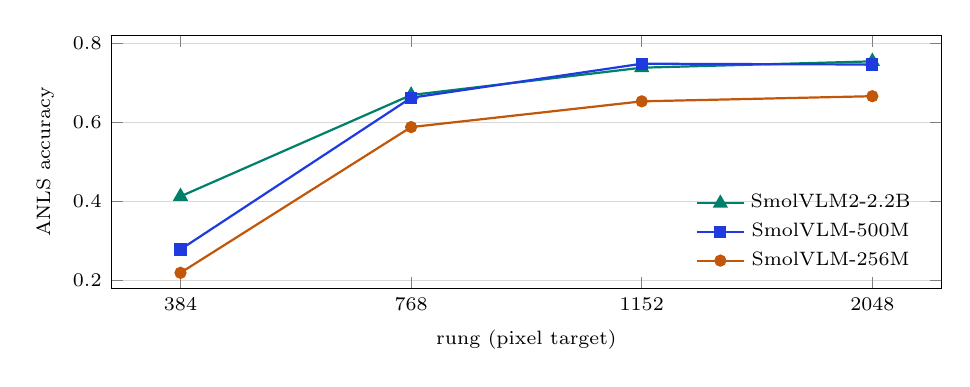
\begin{tikzpicture}
\begin{axis}[
  width=\columnwidth, height=4.8cm,
  xlabel={rung (pixel target)}, ylabel={ANLS accuracy},
  symbolic x coords={384,768,1152,2048}, xtick=data,
  ymin=0.18, ymax=0.82,
  tick label style={font=\scriptsize}, label style={font=\scriptsize},
  legend style={font=\scriptsize,at={(0.98,0.03)},anchor=south east,
                draw=none,fill=none},
  ymajorgrids, grid style={gwelgrid},
]
\addplot[thick,gwelteal,mark=triangle*,mark size=2.4pt] coordinates {
(384,0.413)(768,0.669)(1152,0.738)(2048,0.754)};
\addlegendentry{SmolVLM2-2.2B}
\addplot[thick,gwelblue,mark=square*,mark size=1.8pt] coordinates {
(384,0.279)(768,0.662)(1152,0.748)(2048,0.746)};
\addlegendentry{SmolVLM-500M}
\addplot[thick,gwelorange,mark=*,mark size=1.8pt] coordinates {
(384,0.220)(768,0.588)(1152,0.653)(2048,0.666)};
\addlegendentry{SmolVLM-256M}
\end{axis}
\end{tikzpicture}
\caption{Accuracy against rung on the same $1200$ DocVQA pages. The last step
is flat for all three, though they spend $640$, $640$ and $810$ visual tokens
respectively at the rung where it flattens: the ceiling is a resolution, not a
token budget.}
\label{fig:saturation}
\end{figure}

\paragraph{And the ceiling is a resolution, not a sequence length.} The two
SmolVLM models share an $86$M vision encoder, so ``stops gaining at $1152$\,px''
and ``stops gaining at $640$ visual tokens'' name the same point for both and
cannot be told apart. SmolVLM2-2.2B tokenises differently, spending $810$ tokens
where the others spend $640$, which separates them. All three stop at the same
\emph{pixel} target while spending different numbers of tokens there.
\textbf{What runs out is the information in the pixels, not the sequence length
the model can use.}

\textbf{That makes the saturation point reusable.} It is a property of the
corpus, so it can be found once on the data and carried across a change of
serving model and of vision encoder, which is a far more useful object than a
threshold that must be re-derived per model. We note in fairness that the two
smaller-gap models put a positive point estimate on the top step, leaning the
opposite way from the $500$M; at these interval widths that is noise, and we
report it rather than claim a symmetry the data does not show.

\paragraph{The ladder rule finds the ceiling on its own.} Given rungs and
prices, Eq.~\ref{eq:ladder} selects the top rung on $0\text{--}6\%$ of queries
across the whole preference range: it discovers the saturation from the
calibrated gains without being told. Paired against the binary policy over $30$
resamples of a held-out $300$ (Table~\ref{tab:ladderdocvqa}), it is
significantly cheaper at three of four operating points, and at the highest
preference it is cheaper at accuracy the comparison cannot separate.

\begin{table}[t]
\centering\small
\setlength{\tabcolsep}{4pt}
\begin{tabular}{lcc}
\toprule
$V$ & accuracy delta & latency delta (ms) \\
\midrule
$400$  & $+0.359\ [+0.346, +0.374]$ & $+86.0\ [+84.3, +87.4]$ \\
$800$  & $-0.010\ [-0.019, -0.001]$ & $-161.1\ [-163.9, -158.4]$ \\
$1600$ & $-0.010\ [-0.017, -0.003]$ & $-154.5\ [-158.3, -150.7]$ \\
$3200$ & $-0.002\ [-0.009, +0.005]$ & $\mathbf{-136.4\ [-141.1, -132.0]}$ \\
\bottomrule
\end{tabular}
\caption{Ladder minus binary on $1200$ DocVQA pages, paired within each
operating point over $30$ resamples. At $V=400$ the binary rule barely escalates
at all and the ladder buys $36$ accuracy points for $86$\,ms; above that it
trades at most one accuracy point for roughly $150$\,ms.}
\label{tab:ladderdocvqa}
\end{table}

The mixture measured this effect at $-9.6$\,ms because most of its ladder did
not exist. We report the intervals per operating point rather than pooled across
them: an earlier version of this comparison bootstrapped the four preference
means, which resamples four numbers and yields an interval four points wide.

\paragraph{A refinement of ours that does not pay.} The cost audit suggested an
obvious improvement: since escalation prices vary $2.5\times$ across the pilot,
charge each query its own break-even $\tau_i = \Delta t_i / V$ rather than a
global one. Implemented and measured, it is worth nothing, $+0.000$
$[-0.000,+0.000]$ accuracy and $-1.5\ [-4.3,+0.4]$\,ms, both spanning zero.

The reason is the confound again. Image size is largely a \emph{domain}
property, so within a domain the prices a per-query rule would discriminate
between barely differ, and there is nothing for the refinement to bite on. It
would matter for a router serving one queue of genuinely mixed image sizes, and
we report it as a negative rather than dropping it because the negative is the
informative part: the same fact that makes the probe a domain detector makes
per-query pricing redundant within a domain.

\paragraph{One caveat on the UCCI contrast.} The gap of
Table~\ref{tab:rule}, calibrating correctness over-spending against calibrating the gain, is a mixture effect too. Within a domain both rules land on the front
at different operating points, and the sign flip that separates them is weaker.
We state the contrast as measured on the mixture and unresolved within a domain.

\section{Knowing \emph{whether} is not knowing \emph{where}}
\label{sec:localizer}

Our measurements show region choice matters more than action choice, so we
tested whether the same internal signals locate the region. SmolVLM lays its 64
visual tokens in a contiguous $8\times8$ grid, so the states covering candidate
cell $k$ can be pooled,
\begin{equation}
z_k = \frac{1}{|\mathcal{P}_k|}\sum_{p \in \mathcal{P}_k} h^{(\ell)}_p,
\end{equation}
and ranked by a probe trained on which cells actually answered correctly. This
requires no judge model, no reinforcement learning and no extra forward pass.

On a $2\times2$ grid the localizer scores $48\text{--}51\%$ across six depths
against $51\%$ for choosing uniformly at random, with a $64\%$ oracle ceiling.
Overlapping cells make random choice strong there, so we repeated the experiment
at $3\times3$ and then at $4\times4$. The finer grid is a fairer test: on the
$400$ examples all three share, the gap between random and the oracle widens
from $12.2$ to $16.2$ points as cells shrink, so a localizer has more to find,
not less.

\paragraph{One split is not enough to state a negative.} Our earlier claim,
that at no depth on either grid does the localizer beat random, rests on a
single train/test split. Resampling it $60$ times changes the sign of the
answer (Table~\ref{tab:localizer}).

\begin{table}[t]
\centering\small
\setlength{\tabcolsep}{4pt}
\begin{tabular}{lcc}
\toprule
& $2\times2$ ($n=500$) & $4\times4$ ($n=400$) \\
\midrule
depths beating random & $1$ of $6$ & $\mathbf{4}$ of $\mathbf{4}$ \\
best margin & $+0.006$ & $+0.009\ [0.005, 0.014]$ \\
headroom to the oracle & $0.122$ & $0.162$ \\
share of the gap closed & n/a & $\mathbf{6\%}$ \\
\bottomrule
\end{tabular}
\caption{Localizer margin over random cell choice, $60$ resampled splits.
Random is recomputed on each test fold rather than assumed, since the
cell-correctness rate varies by fold.}
\label{tab:localizer}
\end{table}

At $4\times4$ the localizer beats random at every depth, with intervals
excluding zero. It also beats it by $0.9$ accuracy points, which is $6\%$ of the
gap that a perfect localizer would close. \textbf{The honest claim is about
magnitude, not sign}: the signal is real and it is too small to build on. We
state it that way because we have insisted elsewhere in this paper that a null
is only a result when the interval is tight enough to have found an effect, and
the converse obligation applies here.

\paragraph{What the localizer would have been worth.} A negative result is
easier to accept when the thing that failed is cheap. This one is not. Both
ways of spending a visual-token budget are in the pilot, so they can be put on
one axis (Table~\ref{tab:twoways}): a rung spends its tokens on the whole frame,
a crop spends them on one cell at high magnification. This is also the
comparison \S\ref{sec:cost} has been making against the pruning
literature~\cite{glimpseprune} in words rather than numbers.

\begin{table}[t]
\centering\small
\setlength{\tabcolsep}{4pt}
\begin{tabular}{llcc}
\toprule
family & configuration & tokens & accuracy \\
\midrule
resolution & $384$\,px & $64$ & $0.383$ \\
resolution & $768$\,px & $320$ & $0.516$ \\
resolution & full & $320$ & $0.549$ \\
\midrule
crop, random cell & $2\times2$ & $\mathbf{128}$ & $0.392$ \\
crop, best cell & $2\times2$ & $\mathbf{128}$ & $\mathbf{0.584}$ \\
\bottomrule
\end{tabular}
\caption{Accuracy against visual tokens, $n=1000$, two ways of spending the same
budget. Paired against the best resolution configuration, the best crop is
$+0.035\ [0.008, 0.063]$ more accurate at $2.5\times$ fewer tokens.}
\label{tab:twoways}
\end{table}

\begin{figure}[t]
\centering
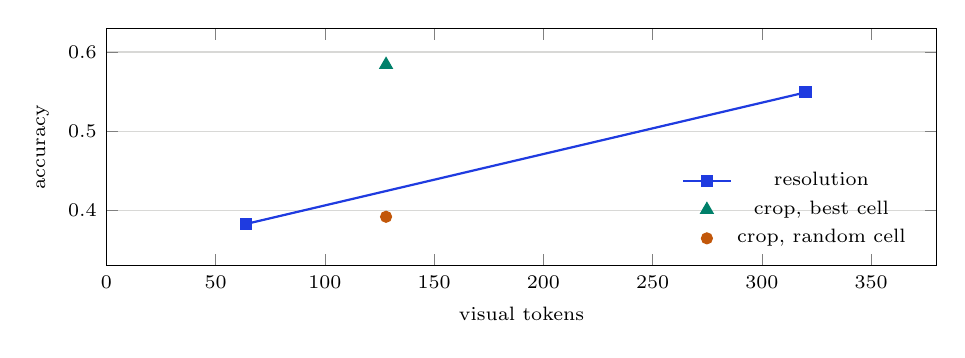
\begin{tikzpicture}
\begin{axis}[
  width=\columnwidth, height=4.6cm,
  xlabel={visual tokens}, ylabel={accuracy},
  xmin=0, xmax=380, ymin=0.33, ymax=0.63,
  tick label style={font=\scriptsize}, label style={font=\scriptsize},
  legend style={font=\scriptsize,at={(0.98,0.03)},anchor=south east,
                draw=none,fill=none},
  ymajorgrids, grid style={gwelgrid},
]
\addplot[thick,gwelblue,mark=square*,mark size=1.8pt] coordinates {
(64,0.383)(320,0.549)};
\addlegendentry{resolution}
\addplot[only marks,mark=triangle*,mark size=2.6pt,gwelteal] coordinates {(128,0.584)};
\addlegendentry{crop, best cell}
\addplot[only marks,mark=*,mark size=2pt,gwelorange] coordinates {(128,0.392)};
\addlegendentry{crop, random cell}
\end{axis}
\end{tikzpicture}
\caption{Two ways to spend a visual-token budget, $n=1000$. The best crop sits
above the resolution line at $2.5\times$ fewer tokens; a randomly chosen one sits
on it. The vertical distance between the two crop markers is what a localizer
would have to recover, and \S\ref{sec:localizer} recovers $6\%$ of it.}
\label{fig:twoways}
\end{figure}

The two readings of the crop row are the whole point (Fig.~
ef{fig:twoways}). A \emph{randomly} chosen
cell reaches $0.392$, which is what the same tokens buy in resolution
($0.383$ at $64$, and about $0.42$ interpolated at $128$). The \emph{best} cell
reaches $0.584$, beating the dearest resolution configuration while spending
$2.5\times$ fewer tokens. \textbf{Position is worth more per token than
resolution, and only to a policy that knows where to look.}

That prices the failure. A working localizer would be the most token-efficient
action in this action space, which is presumably why~\cite{awares} is willing to
spend cold-start fine-tuning, multi-turn GRPO and a $70$B judge to obtain one.
Our $0.9$-point margin buys none of that headroom.

The low-resolution pass knows \emph{whether} more resolution would help and
essentially not \emph{where} to spend it. This bounds what internal signals
deliver at this scale, and suggests that the supervision machinery
of~\cite{awares} is not overengineering.

\section{Limitations}

Three serving models, one GPU, and two pilots: $1000$ examples across four
datasets and $1200$ within one, the latter run on all three. The saturation
ceiling is the claim we have pushed hardest, over an $8.6\times$ parameter range
and two distinct vision encoders, and it has not moved. What we cannot say is
whether it would move for a family trained differently: all three models come
from one lineage and one data recipe, so a shared pretraining corpus remains a
possible common cause. Our strongest baseline is
the published escalation \emph{mechanism} without its training; a re-implemented
VisionThink at sub-1B scale remains the comparison the field would want, and the
gap between an untrained self-report and a trained one is exactly what we cannot
measure.

Four limitations deserve more than a mention. The latency saving needs an
inference stack that can abandon a prefill mid-flight and start a different
image. We verified this is real rather than arithmetic: physically truncating
the decoder to its first six layers gives a $20.5$\,ms prefill, within $1\%$ of Eq.~\ref{eq:probecost}'s prediction, and an escalated query then costs
$277.0$\,ms against $402.9$\,ms for completing the cheap pass first, a measured
$31\%$ saving. What standard serving frameworks do not expose is the
\emph{control} to do this per query, so the saving is available but not yet
convenient. Absolute accuracies run from
$0.385$ to $0.580$, a regime where the model is wrong about half the time, and
conclusions drawn there may not transfer to a model that is usually right. The
probe's direction does not transfer across question domains (trained on detail-limited data and tested on knowledge-limited data it scores $0.422$, and the reverse $0.366$, both below chance) so deployment needs a
domain-representative calibration set and a shift detector. And the cross-model
transfer result uses two models that share an identical $86$M vision encoder,
so part of what transfers may be encoder-side rather than genuinely
cross-model; separating those requires a source model with a different encoder.

We ask many questions of one dataset mixture, so the intervals above are
corrected rather than nominal. Thirteen paired comparisons at the nominal $5\%$
level carry a $49\%$ chance of at least one false positive, so we convert each
bootstrap to a two-sided p-value and run Holm's step-down over the family.
Nothing is lost: the nine comparisons that clear the nominal level are the same
nine that survive correction, at adjusted $p = 0.0013$, because the surviving
effects sit at the bootstrap's resolution floor while the failures are
unambiguous nulls.

The split is itself informative. \textbf{Every surviving comparison is about
cost}; all three probe-versus-entropy \emph{accuracy} comparisons fail, as does
the top rung's gain. That is the paper's claim structure certified rather than
asserted: what we demonstrate is cheaper compute at accuracy the data cannot
separate, not better answers.

The Pareto-dominance result is the one we have tested hardest and it came back
qualified: universal dominance holds on the reported fold and in $52\%$ of
resplits, so the claim we make is the distributional one ($90\%$ of the front, a
saving positive in $200$ of $200$ splits) and not the categorical one. Readers
should treat any single-fold dominance statement in this literature, including
our own earlier one, as untested until resampled.

One limit is specific to \S\ref{sec:rule}: $V$ is elicited, not measured, so the
contribution is that the policy is determined \emph{given} a preference, not
that we know the preference. The adversarial result is a proxy: it shows the probe is not
incidentally moved by what moves entropy, not that it resists an attack
optimised against it.

The confound audit of \S\ref{sec:confound} has a limit of its own, in our
favour and worth stating. Fitting inside one dataset gives the probe $210$
training examples where the pooled fit gets $600$, so part of the collapse could
be sample size rather than absent signal. Two observations argue against that
reading (entropy needs no training at all and is therefore unaffected, and the probe is at or below chance rather than merely noisy) but the clean test is a
single-domain corpus large enough to fit and test inside, and $300$ examples per
dataset is not it. We report the confound as established and its magnitude as
uncertain.

\section{Reproducibility}

Every numeric claim in this paper is re-derived from the run records by a
validation harness with an explicit threshold per claim, which exits non-zero if
any stops holding; it currently checks fifty-six, including the negative
results on localization, on our own energy instrument, and on the universality
of Pareto dominance, that last one asserts the claim is \emph{not} universal,
so restating it too strongly fails the build. Claims stated in the text and
not covered by a check are marked as unverified. The oracle runs are stored as
append-only JSONL with per-configuration answers, generation scores and hardware
measurements, so correctness metrics and cost weights can be changed offline
without re-running any model. Splits are hash-based on example identifiers, so
growing the pilot never reshuffles examples already assigned.

\paragraph{Compute.} Every experiment in this paper runs on one RTX 4060 laptop
GPU with $8.6$\,GB of memory. The oracle runs comprise $54\,660$
instrumented generations totalling $305$ minutes of measured model time, of
which the $1200$-page single-domain pilot is $6\,000$ generations per serving
model, $40$ minutes each for the two SmolVLM models and $54$ for SmolVLM2-2.2B; activation extraction and the component profiles add roughly a further
half hour. Wall-clock is appreciably larger, since image decoding, the
processor, and the instrumentation itself sit outside the timed region. No
training of any kind was performed: every probe here is a difference of means
over cached activations, and every calibration a single isotonic pass, both of
which take seconds on a CPU. The reproduction cost of this paper is therefore
about six GPU-hours, which is the point of working at this scale.

\section{Conclusion}

We set out to ask what a 500M vision--language model knows about its own need
for more pixels before it generates anything. The answer we can defend is
narrower than the one we expected, and arriving at it was the useful part.

On a four-dataset mixture, a linear probe on pre-generation activations ranks
escalation value better than output confidence and yields a policy readable
after a sixth of the language model. Inside any one of those datasets it reaches
$0.572$ where output confidence, fitted on nothing, reaches $0.663$, and more
training data narrows that gap without closing it. What the direction mostly
encodes is which \emph{kind} of image is present: a quantity that predicts
escalation value across a benchmark mixture, because the mixture's datasets
differ enormously in how much resolution buys, and predicts much less within
one. Raw image size, free to read, captures almost all of it.

Two things bound the claim rather than one. This is a way of deciding
\emph{whether} to look again and not \emph{where}, and on the evidence here it
is a way of deciding for a heterogeneous mixture and not for a workload.

What we would keep is the part that did not depend on the probe. The decision
rule is signal-agnostic and survives on output confidence, where one stated
preference produces a different escalation rate per domain without retuning. And
the resolution ladder turns out to carry most of the money that was attributed
to the escalate/answer decision: on document pages, $93\%$ of what escalation
repairs is repaired below the top rung, and the ceiling sits at a pixel
resolution that three models with two vision encoders agree on.

The result we would most like others to carry away is the negative one in
\S\ref{sec:policy}, which we encountered four times. A probe trained on the
conditional target beat its baseline on ranking and lost the policy comparison
by $8.5$ points. An ensemble of entropy and probe then beat both on ranking and
lost the policy comparison on cost. A rule calibrating the weak pass's error
probability, which is the standard cascade recipe, matched our accuracy while
spending $59\%$ relatively more compute. And the signal that beat all of them on
the mixture turned out to be ranking the mixture. The target was wrong, then the
signal was too expensive to read, then the calibration target was wrong, then
the evaluation distribution was doing the work. None of the four is visible in
an AUROC table.

Reporting ranking quality without building the policy is reporting the wrong
number. The four ways of getting it wrong are optimising a target the policy
does not face, optimising a signal the policy cannot afford, calibrating a
quantity whose assumptions the setting violates, and reading a between-group
difference as a within-group one. All are easy to miss.

The last is the one we would flag most broadly, with the caveat that the
literature we borrowed the probe from had already avoided it: any probe
evaluated on a mixture of benchmarks that differ in the outcome being predicted
should be scored within each of them before it is believed. The text-routing
work reports per-dataset AUROC and warns explicitly about directions that
capture dataset-specific cues~\cite{cencerrado}; we pooled, and pooling is what
produced our headline. The check costs one line, and it was our own evaluation
protocol rather than the method that failed it.


\appendix

\section{What each part is worth}
\label{sec:ablation}

The components above are each justified where they are introduced, over five
sections and on folds and cost models that were not always identical. That is
how a paper acquires an inconsistency it cannot see, so we recompute all of them
against one reference on one fold with one cost model.

\paragraph{Read at a fixed preference, an ablation says the opposite of the
truth.} Our first attempt held $V$ constant and compared raw accuracy. Every
removal appeared to \emph{improve} accuracy, because every removal escalated
more, and at fixed $V$ nothing prevents a variant from buying accuracy with
latency. That is the error this paper spends \S\ref{sec:policy} warning about,
committed on ourselves. Each variant is therefore swept to a frontier and read
at a fixed latency budget (Table~\ref{tab:ablation}).

\begin{table}[t]
\centering\small
\setlength{\tabcolsep}{4pt}
\begin{tabular}{lcc}
\toprule
variant & acc.\ at $400$\,ms & acc.\ at $500$\,ms \\
\midrule
\textbf{reference} & $\mathbf{0.653}$ & $\mathbf{0.743}$ \\
no per-example pricing & $0.650\ (-0.003)$ & $0.744\ (+0.000)$ \\
no calibration (tuned rate) & $0.431\ (-0.221)$ & $0.571\ (-0.172)$ \\
no ladder (binary) & $0.281\ (-0.372)$ & $0.622\ (-0.121)$ \\
no gain target (UCCI) & $0.278\ (-0.375)$ & $0.611\ (-0.133)$ \\
no signal (fixed policy) & $0.278\ (-0.375)$ & $0.278\ (-0.465)$ \\
\bottomrule
\end{tabular}
\caption{Each variant swept over six operator preferences and read at a fixed
budget, $1200$ DocVQA pages, $30$ resamples. Deltas are paired against the
reference frontier.}
\label{tab:ablation}
\end{table}

Three things. The losses are real but wildly unequal, so the table is a ranking
of what matters rather than a list of things that help. \textbf{At $400$\,ms the
ladder is what makes the budget usable at all}: binary escalation reaches
$0.281$, which is always-cheap to within $0.003$, because no binary policy can
afford the top rung inside that budget. And per-example pricing costs $-0.003\
[-0.004, -0.001]$: an interval excluding zero, so a real effect, and small
enough that we report it as negligible rather than as nothing. Those are
different claims and the check that guards this table asserts the second.


\section{A second serving model, and cross-model transfer}
\paragraph{Replication on a second serving model.} Every result above has one
model deciding for itself, so we repeated the entire chain (oracle run, activation extraction, probe fitting, rate sweep) with SmolVLM-256M as the
model that answers, on the same $1000$ images and questions
(Table~\ref{tab:replication}).

\begin{table}[t]
\centering\small
\setlength{\tabcolsep}{4pt}
\begin{tabular}{lcccc}
\toprule
serving & cheap & full & probe & entropy \\
model & acc. & acc. & AUROC & AUROC \\
\midrule
SmolVLM-500M & $0.383$ & $0.549$ & $0.761$ & $0.751$ \\
SmolVLM-256M & $0.298$ & $0.511$ & $0.682$ & $0.616$ \\
\bottomrule
\end{tabular}
\caption{AUROC is on the joint escalation-gain target. On the reported fold of
both models every entropy operating point is Pareto-dominated; six probe points
lie on the front for the 256M model, four for the 500M. The resplit test of
Fig.~\ref{fig:resplit} was run for the 500M model only.}
\label{tab:replication}
\end{table}

The finding replicates and strengthens. On the smaller model the probe's
advantage on the joint target widens from $+0.010$ to $+0.066$, and at the
highest escalation rate both signals reach $0.455$ accuracy while the probe
costs $190.3$\,ms against $278.0$\,ms, $32\%$ less, against $12\text{--}22\%$
on the 500M.

Two properties survive the halving of model size and one does not.
Self-knowledge is unchanged: AUROC on ``will the cheap pass be correct'' is
$0.751$ against $0.758$, a difference of seven thousandths for a model with
half the parameters and $16$ fewer accuracy points. The escalation
\emph{opportunity} also grows, escalation repairs $24\%$ of queries against
$21\%$, and damages $3\%$ against $4\%$. But knowing whether escalation will
help degrades, from $0.734$ to $0.672$: half of the smaller model's failures are
unsolvable at any resolution, so the recoverability signal has less to work
with. A weaker model needs routing more and can route slightly less well.

\paragraph{Cross-model transfer.} Following the Encoder--Target Decoupling of
\cite{llmrouter}, we predict the 500M model's escalation outcomes from
SmolVLM-256M activations on the same images. This scores $0.785\ [0.692,
0.873]$ at layer 30 and $0.770$ at layer~1: at least as well as the 500M model
predicts its own. The probe can therefore run off the serving path entirely, on
a separate model that can be batched or placed on different hardware.


\section{An adversary on the allocation signal}
\paragraph{The signal an attacker cannot see.} A routing rule is an attack
surface. Liu et al.~\cite{deferral} force deferral in multimodal cascades with a
border-confined trigger that flattens the weak model's output distribution,
inflating the provider's bill without changing any accuracy metric. Their attack
is metric-agnostic precisely because it targets that distribution, which the
probe never reads. As a cheap proxy we applied unoptimised border perturbations
covering $36\%$ of the image, with the probe fitted on training examples only
(Table~\ref{tab:attack}).

\begin{table}[t]
\centering\small
\begin{tabular}{lccc}
\toprule
perturbation & signal & shift & escalation \\
\midrule
high-frequency noise & entropy & $+0.28\sigma$ & $50\% \to \mathbf{62\%}$ \\
high-frequency noise & probe   & $-0.04\sigma$ & $50\% \to 50\%$ \\
flat fill            & entropy & $+0.19\sigma$ & $50\% \to \mathbf{56\%}$ \\
flat fill            & probe   & $+0.01\sigma$ & $50\% \to 50\%$ \\
\bottomrule
\end{tabular}
\caption{Border perturbations touching no central pixel, $80$ held-out images.
Two structurally opposite perturbations both raise output entropy and neither
moves the probe.}
\label{tab:attack}
\end{table}

A perturbation requiring no optimisation, no model access and no knowledge of
the deployed metric inflates compute by $24\%$ relative when allocation reads
output entropy, and by nothing when it reads the probe. We claim only the weak
form: an attacker optimising the output distribution is not optimising a
projection onto a direction they cannot observe, and here that indirection
suffices. A white-box attacker who knows the probe direction is the case this
does not settle.


\section{Abstention as a third action}
\label{sec:abstain}

We defined three targets in \S\ref{sec:two-questions} and have used two.
$Q_3$ (answerable at all?) is negative for $30.6\%$ of the pilot: no
configuration we run answers those queries correctly. A system that could
recognise them would decline instead of spending, which is the third action the
efficiency literature omits and the selective-prediction literature is built
around~\cite{abstention,recoverr}. Two axes decide whether it is worth adding,
and they disagree.

\paragraph{As a way to hold risk down, abstention is the weaker lever.} Under a
risk constraint the alternative to declining is to spend more and re-decide.
Sweeping both thresholds and charging escalated queries for both passes
(Table~\ref{tab:coverage}), escalation reaches coverage that abstention cannot.

\begin{table}[h]
\centering\small
\begin{tabular}{lccc}
\toprule
risk tolerance & abstain only & or escalate & cost \\
\midrule
$\le 30\%$ & unreachable & $\mathbf{58\%}$ & $320.8$ \\
$\le 40\%$ & $41\%$ & $\mathbf{88\%}$ & $312.2$ \\
$\le 50\%$ & $69\%$ & $\mathbf{100\%}$ & $200.7$ \\
\bottomrule
\end{tabular}
\caption{Maximum coverage at each risk tolerance, latency in milliseconds. At a
$30\%$ tolerance abstention alone serves no query at acceptable risk.}
\label{tab:coverage}
\end{table}

At a $50\%$ tolerance escalation reaches full coverage while escalating $38\%$
of traffic. The comparison needs a cost-instrumented multi-configuration run,
which is the artefact the efficiency literature builds and the
selective-prediction literature does not, and it says the two fields have been
pulling different levers on the same signal.

\paragraph{As a way to save compute, abstention is nearly worthless
here, because the rule got there first.} Escalating a query no configuration
can answer is pure waste, and $30.0\%$ of the test fold is in that state. If the
gain rule of \S\ref{sec:rule} spent its escalation budget blind to solvability,
a perfect abstention gate would recover that entire share. It does not
(Table~\ref{tab:abstain}).

\begin{table}[h]
\centering\small
\begin{tabular}{lccc}
\toprule
$V$ & escalates & of which hopeless & perfect gate saves \\
\midrule
$400$  & $24\%$ & $17\%$ & $2.8\%$ \\
$800$  & $34\%$ & $19\%$ & $4.2\%$ \\
$1600$ & $40\%$ & $22\%$ & $5.3\%$ \\
\bottomrule
\end{tabular}
\caption{Escalation is aimed below the $30.0\%$ base rate of unsolvable
queries, so an oracle abstention gate (which cannot lose accuracy, since those queries are wrong under every action) recovers only the margin.}
\label{tab:abstain}
\end{table}

Calibrating on the signed gain already suppresses these queries: they have
$\mathbb{E}[G \mid x] \approx 0$ whatever their error probability, so the rule
declines them for the same reason it declines confident failures. The residual
headroom for a perfect, free abstention detector is $4.2\%$ of latency at
$V=800$. \textbf{A third action is not where the remaining budget is.} What the
escalation budget actually buys is visible in the same run: $54\%$ of escalated
queries have zero gain, escalation changes nothing, and that, not
unanswerability, is the waste worth attacking.

\paragraph{If a guarantee is needed rather than a preference.} Both
\S\ref{sec:rule}'s rule and the thresholds above are calibrated to a point
estimate. Where an operator needs a distribution-free promise instead, the
three-way split of~\cite{conformal} transfers directly, with its middle regime
spending compute rather than widening a prediction set: at answer-level
$\alpha = 0.5$ the policy answers $52\%$, escalates $38\%$ and declines $9\%$,
and its coverage guarantee holds out of sample to within $+0.025$. A recall
floor in the style of~\cite{recall} gives the complementary guarantee (retain at least $90\%$ of the queries escalation would have fixed, achieved $97\%$ on the test fold) and cannot collapse to never escalating by construction, which
is the failure mode our cost-minimising tuners exhibited. We report these as
available machinery rather than as our headline policy, since neither improves
on the cost-derived rule when a preference can be stated.


\begin{thebibliography}{9}\small
\bibitem{visionthink} S.~Yang et al. VisionThink: Smart and Efficient Vision Language Model via Reinforcement Learning. arXiv:2507.13348, 2025.
\bibitem{adaptvision} Z.~Lin et al. AdaptVision: Efficient Vision-Language Models via Adaptive Visual Acquisition. arXiv:2512.03794, 2026.
\bibitem{awares} N.~Shabtay et al. Look Where It Matters: High-Resolution Crops Retrieval for Efficient VLMs. arXiv:2603.16932, 2026.
\bibitem{glimpseprune} Q.-S.~Zeng et al. A Glimpse to Compress: Dynamic Visual Token Pruning for Large Vision-Language Models. arXiv:2508.01548, 2025.
\bibitem{lugoloobi} W.~Lugoloobi et al. LLMs Encode Their Failures: Predicting Success from Pre-Generation Activations. arXiv:2602.09924, 2026.
\bibitem{cencerrado} I.~V.~Moreno Cencerrado et al. No Answer Needed: Predicting LLM Answer Accuracy from Question-Only Linear Probes. arXiv:2509.10625, 2026.
\bibitem{llmrouter} T.~Varshney et al. LLM Router: Rethinking Routing with Prefill Activations. arXiv:2603.20895, 2026.
\bibitem{energy} J.~Zhan et al. Seeing is Free, Speaking is Not: Uncovering the True Energy Bottleneck in Edge VLM Inference. ACM MM, 2026.
\bibitem{smolvlm} A.~Marafioti et al. SmolVLM: Redefining small and efficient multimodal models. arXiv:2504.05299, 2025.
\bibitem{quantization} H.~Shin et al. Rethinking Small VLM Quantization: From Component-Wise Analysis to Hardware-Aware Edge Deployment. ICML Workshop, 2026.
\bibitem{ucci} V.~Kotte. UCCI: Calibrated Uncertainty for Cost-Optimal LLM Cascade Routing. arXiv:2605.18796, 2026.
\bibitem{recall} Ruan et al. Doomed from the Start: Early Abort of LLM Agent Episodes via a Recall-Controlled Probe Cascade. arXiv:2607.06503, 2026.
\bibitem{conformal} K.~Tayebati et al. Learning Conformal Abstention Policies for Adaptive Risk Management in Large Language and Vision-Language Models. arXiv:2502.06884, 2025.
\bibitem{clusterroute} Moslem et al. Cluster, Route, Escalate: Cascaded Framework for Cost-Aware LLM Serving. arXiv:2606.27457, 2026.
\bibitem{deferral} Liu et al. Forced Deferral: Manipulating Routing Decisions in Multimodal LLM Cascades. arXiv:2606.15308, 2026.
\bibitem{cascadefail} Sun et al. When Efficiency Backfires: Cascading LLMs Trigger Cascade Failure under Adversarial Attack. arXiv:2605.17288, 2026.
\bibitem{vlcache} Y.~Wang et al. VLCache: Computing 2\% Vision Tokens and Reusing 98\% for Vision-Language Inference. arXiv:2512.12977, 2026.
\bibitem{abstention} Knowing When Not to Answer: Evaluating Abstention in Multimodal Reasoning Systems. arXiv:2604.14799, 2026.
\bibitem{recoverr} Srinivasan et al. Selective ``Selective Prediction'': Reducing Unnecessary Abstention in Vision-Language Reasoning. arXiv:2402.15610, 2024.
\end{thebibliography}

\end{document}
